%\documentclass[10pt,draftclsnofoot,journal,a4paper,oneside,onecolumn]{IEEEtran}
\documentclass[10pt,final,journal,a4paper,oneside,twocolumn]{IEEEtran}
\usepackage[english]{babel}
\usepackage[T1]{fontenc}
\usepackage[latin1]{inputenc}
\usepackage[]{graphicx}
\usepackage{amssymb,amsmath}
\usepackage{tikz}
\usepackage{circuitikz}
\usepackage{lipsum}

% Additional packages required by the ported report content
\usepackage{mathtools}
\usepackage{booktabs}
\usepackage{array}
\usepackage{ragged2e}
\usepackage{textcomp}
\usepackage{url}
\usepackage{enumitem}
\newcolumntype{L}[1]{>{\RaggedRight\arraybackslash}p{#1}}

\ifCLASSOPTIONcompsoc
\usepackage[caption=false,font=normalsize,labelfont=sf,textfont=sf]{subfig}
\else
\usepackage[caption=false,font=footnotesize]{subfig}
\fi

\title{Formula E Interior Permanent Magnet Motor Design\\
{\large Improvement of the Formula Student Team Car's Performance}}

\author{\IEEEauthorblockN{Rene Orlando Garcia Torres\IEEEauthorrefmark{1}, Qirui Zhang\IEEEauthorrefmark{1}}

\IEEEauthorblockA{\IEEEauthorrefmark{1}Kungliga Tekniska h\"ogskolan (KTH), Stockholm, Sweden\\
E-mail: reneogt@kth.se, zhangq@kth.se}
}

\begin{document}

\renewcommand{\figurename}{Fig.}
\renewcommand{\tablename}{Tab.}
\newcommand{\sectionname}{Sect.}

\maketitle

\begin{IEEEkeywords}

Interior permanent magnet machine, V-shape rotor, fractional-slot concentrated winding, field weakening, reluctance torque, analytical sizing, finite element analysis, traction motor, Formula Student.

\end{IEEEkeywords}

\begin{abstract}
This report documents the analytical design and finite-element validation of a new interior permanent magnet (IPM) traction motor intended to replace the DD5-14-10-POW machine used by the KTH Formula Student car. Starting from the existing 10-pole/12-slot topology and its inverter-limited 1.1 flux-weakening ratio, boundary requirements are defined and a V-shape IPM rotor targeting $L_q>L_d$ for added reluctance torque is sized. Two independent Esson's-rule estimates bracket a feasible bore and stack-length envelope, and the full Di Gerlando and Ricca sizing procedure is implemented in MATLAB to produce a complete geometry, winding and rated operating point. The converged design is pushed into a prebuilt COMSOL model for a coupled electromagnetic and structural transient study, and an analytical loss model provides an efficiency map. The design is structurally safe with margin; a no-load leakage-model gap that drives a flux-linkage and torque shortfall is identified as the main open item.
\end{abstract}

\section{Background: Current Motor and Inverter Analysis}
\label{SEC:Background}
The KTH Formula Student team has an already working racing car that has been used in different competitions. This section analyses both Motor and Inverter in order to define a baseline for the new design, focusing on reducing the current motor's limitations and improving the overall performance, tailored to the needs of the team.

\subsection{Motor}
\label{sec:current_motor_background}
The team currently utilizes 4 \textbf{DD5-14-10-POW-18600-B5} motors to power their vehicle. This vehicle is used in different competitions with different terrains. From a flat long track where speed is needed, to auto-cross scenarios where torque is critical. Due to that reason, the car should be able to perform in a variety of conditions. From data-sheets~\cite{DatasheetDD5} and pictures (\figurename~\ref{fig:stator_stator_rotor}), the following characteristics were identified:
\\\textbf{Winding Configuration:} 86 wire ends, indicating a total number of turns per tooth of 43. See \figurename~\ref{fig:stator_stator_rotor} (left).
\\\textbf{Slot Number:} 12 slots, which gives a slot per pole ratio of 1.2 (12 slots / 10 poles), indicating a non-integer slot winding configuration. See \figurename~\ref{fig:stator_stator_rotor} (center).
\\\textbf{Rotor Topology:} Interior permanent magnet (IPM) topology. See \figurename~\ref{fig:stator_stator_rotor} (right): no magnets glued to the rotor surface are visible. The topology cannot be confirmed from the datasheet alone, and it is a possibility that the motor is actually SPM with a slight rotor anisotropy, and the magnets are hard to see. Nevertheless, for the rest of the report we treat it as IPM.
\\\textbf{Saliency Profile:} $L_d = 0.24$ mH and $L_q = 0.12$ mH ($L_q < L_d$).
\\\textbf{Stack Length ($l_e$):} \textbf{85.2 mm}, from the mechanical drawing \cite{DrawingDD5} (\figurename~\ref{fig:side_technical_drawing}, left: $12.4+61+11.8\,\text{mm}$).
\\\textbf{Stator Outer Diameter ($D_{os}$):} \textbf{89.9 mm}, from the mechanical drawing; housing diameter - 3\,mm minimal wall thickness. \cite{DrawingDD5} (\figurename~\ref{fig:side_technical_drawing}, right: $95.9 - 2(3) = 89.9\,\text{mm}$).
\\\textbf{Stator Inner Diameter ($D_{is}$):} \textbf{unknown}. No drawing dimensions the bore.

\begin{figure*}[!t]
    \centering
    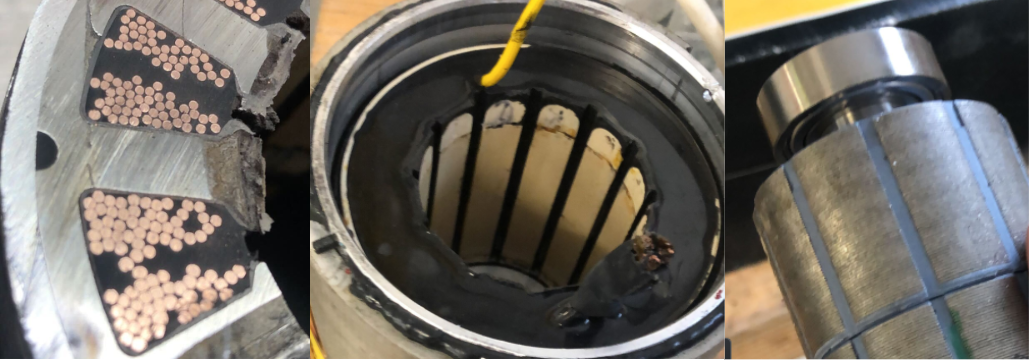
\includegraphics[width=0.8\textwidth]{figures/stator_stator_rotor.png}
    \caption{\textit{Left:} Traversal cut of the stator. \textit{Center:} Stator. \textit{Right:} Rotor.}
    \label{fig:stator_stator_rotor}
\end{figure*}

Note that the same motor/inverter configuration is used for the 4 wheels, but the team considers an uneven power distribution (80/20) between axles for vehicle dynamics purposes; this design still sizes each motor to the full per-wheel spec in \tablename~\ref{tab:propulsion_motor_requirements} (a conservative choice, since the 80/20 split would only ever demand \emph{less} than that from an individual corner), so the distribution itself isn't discussed further in this report.

\begin{figure*}[!t]
    \centering
    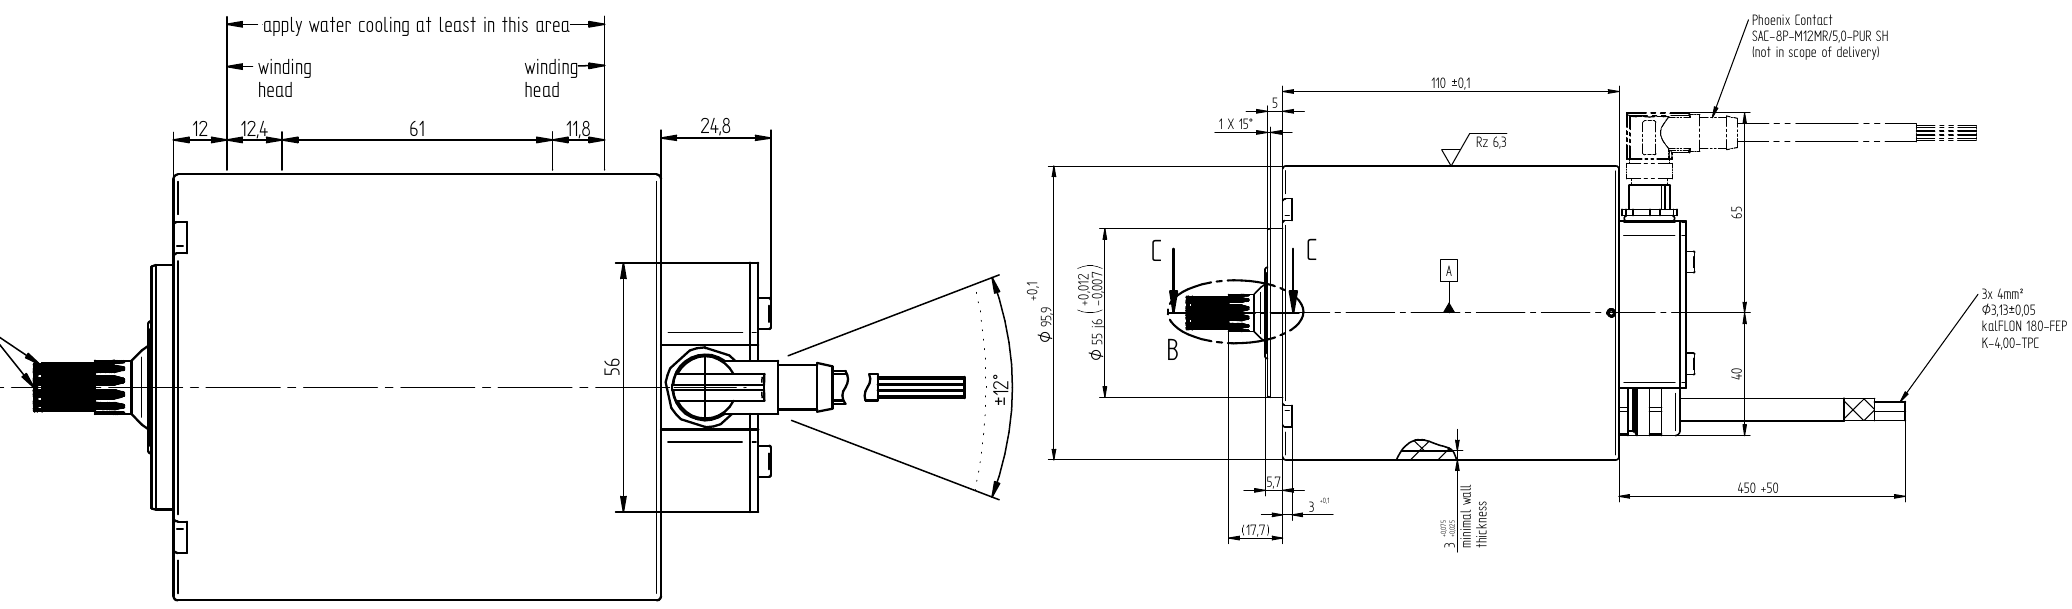
\includegraphics[width=\textwidth]{figures/side_technical_drawing.png}
    \caption{Side view of the current motor.}
    \label{fig:side_technical_drawing}
\end{figure*}

\begin{figure}[!htbp]
    \centering
    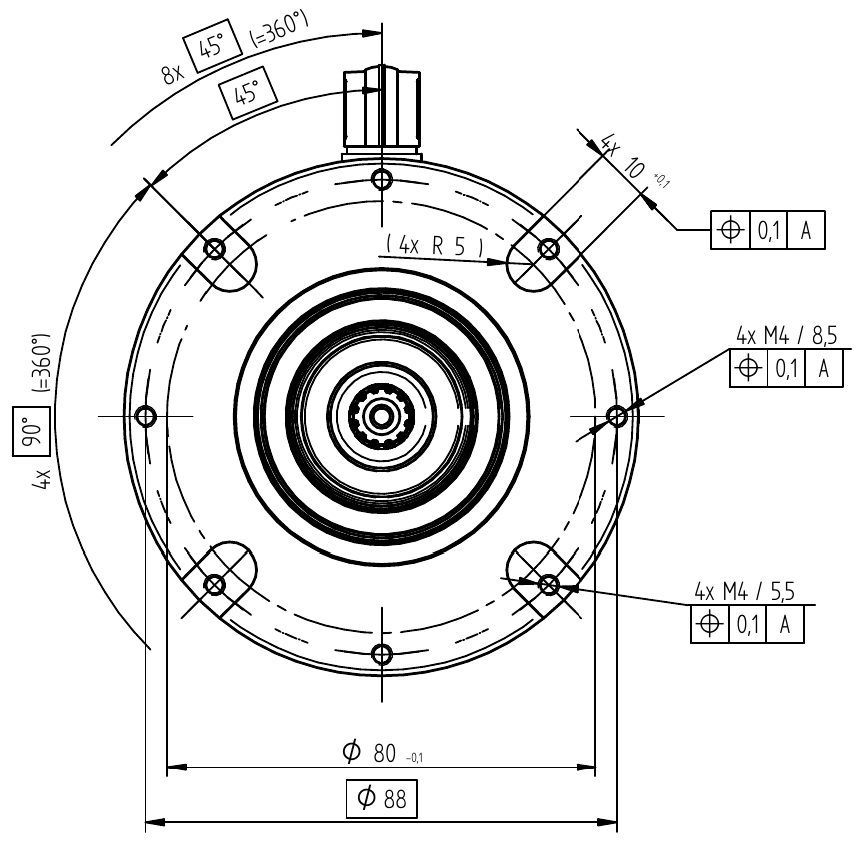
\includegraphics[width=\columnwidth]{figures/front_technical_drawing.png}
    \caption{Front view of the current motor.}
    \label{fig:front_technical_drawing}
\end{figure}

Moreover, each motor is connected to a fixed gearbox with a 14:1 ratio, which will be kept for the new design. Thus, any further speed calculation has to consider that the motor rotates 14 times faster than the wheel. Also, note from \figurename~\ref{fig:power_and_torque_current_motor_mod} how the current motor can operate in field-weakening mode only from 13,200 rpm up to the 20,000 rpm limit, meaning the machine has a ``Flux-weakening ratio'' of 1.52 (20,000 rpm / 13,200 rpm). We will briefly see in \sectionname~\ref{sec:Inverter} that the KW26-S5-FSE-4Q inverter only allows for a max.\ speed of 14,400 rpm, thus leaving a real flux-weakening ratio of only 1.1 (14,400 rpm / 13,200 rpm). For the new design, we aim to increase this ratio up to a value around 1.2.

\begin{figure}[!htbp]
    \centering
    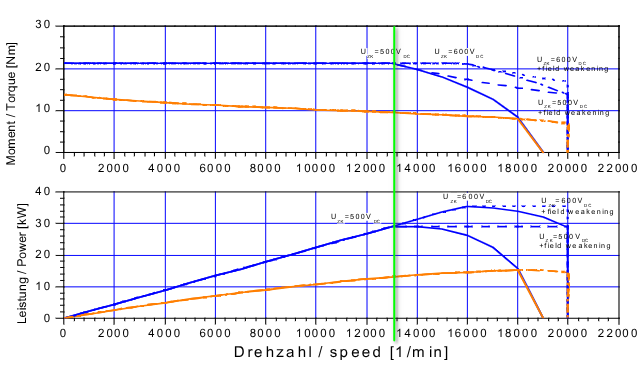
\includegraphics[width=\columnwidth]{figures/power_and_torque_current_motor_mod.png}
    \caption{From datasheet: Power and Torque vs Speed for the current motor. We focus on the $U=500\,V_{DC}$ blue line. The green line marks the knee point where the motor enters field-weakening mode.}
    \label{fig:power_and_torque_current_motor_mod}
\end{figure}

\subsection{Inverter}
\label{sec:Inverter}
The inverter used to drive this motor is the \textbf{KW26-S5-FSE-4Q}. This inverter consists of 4 independent channels.
Notice how the inverter is a bottleneck in this configuration, since the 1200 Hz limit gives a 14,400 rpm for a 10-pole machine. This means that the motor enters field-weakening mode only on the last 10\% range of operation. Here we state the first deviation; \tablename~\ref{tab:propulsion_motor_requirements} states that the Maximum Speed should be 20,000 rpm, but the existing inverter caps the maximum speed at 14,400 rpm. Replacing the inverter is kept out of scope for study.

Throughout this report the DC-link voltage is taken as $V_{DC}=515\,\text{V}$, the assumed nominal for the car's tractive-system bus. AMK documents the DD5 itself at $U_{ZK}=500\,\text{V}$ and $600\,\text{V}$ DC (\figurename~\ref{fig:power_and_torque_current_motor_mod} reads the $500\,\text{V}$ curve); every $V_{DC}$-dependent result in Part A (corner speed, \sectionname~\ref{sec:corner_speed}; winding turns, \sectionname~\ref{sec:stator_winding_sizing}; the current-limit check, \sectionname~\ref{sec:part_b_fea}) derives from this single value.

The following table summarizes the previously analyzed motor/inverter parameters.

\begin{table}[!t]
\centering
\caption{Current motor parameters (DD5-14-10-POW)}
\label{tab:current_motor_data}
\begin{tabular}{@{}L{0.44\columnwidth} L{0.19\columnwidth} L{0.26\columnwidth}@{}}
\hline
\textit{Parameter} & \textit{Symbol} & \textit{Value}\\ \hline
\textbf{Pole Number} & $P$ & 10 \\
\textbf{Slot Number} & $N_s$ & 12 \\
\textbf{DC-link Voltage} & $V_{DC}$ & 515 V\\
\textbf{Nominal Power} & $P_{n}$ & 12.3 kW \\
\textbf{Peak Power} & $P_{max}$ & 28 kW \\
\textbf{Nominal Torque} & $M_{n}$ & 9.8 Nm \\
\textbf{Nominal Speed} & $N_{n}$ & 12,000 rpm \\
\textbf{Max. Speed} & $N_{max}$ & 14,400 rpm \\
\textbf{Corner Speed Point} & $N_{char}$ & 13,200 rpm \\
\textbf{Gear Ratio} & $G$ & 14:1 \\
\textbf{Stack Length} & $l_e$ & 85.2 mm \\
\textbf{Stator Outer Diameter} & $D_{os}$ & 89.9 mm \\
\textbf{Aspect ratio (housing-referenced)} & $l_e/D_{housing}$ & 0.888 \\ %TODO: Assess if this is actually a valuable ratio.
\textbf{Flux-weakening Ratio (inverter constrained)} & $N_m/N_c$ & 1.1 \\
\textbf{Rotor Topology} & n/a & Interior Permanent Magnet \\ \hline
\end{tabular}
\end{table}

\section{Part A: Requirements Definition And Analytical Design}
\label{SEC:PartA}
This section will define the initial values and limitations that will guide the design of the new motor. Then, using different analytical methods, we will reach some design results without simulation. After this iteration, we will use FEA to validate the design and iterate until we reach a final design that meets the requirements.

\subsection{Boundary Requirements}
The following table summarizes the design boundaries, which are constrained by the inverter properties, mechanical enclosure and the Formula Team itself. The new design should stick to these requirements, and any design deviation should be justified.

\begin{table*}[!t]
\centering
\caption{Boundary requirements for the new propulsion motor design.}
\label{tab:propulsion_motor_requirements}
\begin{tabular}{@{}L{0.42\linewidth}L{0.32\linewidth}@{}}
\toprule
\multicolumn{2}{@{}l@{}}{\textbf{General requirements}} \\
\midrule
Max dimensions including cooling (outer diameter $\times$ length) & 120 mm $\times$ 110 mm \\
Hub compatible & Must \\
Motor topology & Radial in-runner (rotor inside the stator) \\
Weight & $\leq$ 2800 g \\
Power density (mass) & $\geq$ 10 kW/kg \\
IP protection & IP65 \\
\addlinespace
\multicolumn{2}{@{}l@{}}{\textbf{Mechanical requirements}} \\
\midrule
Peak torque (for 5 s) & 21.5 Nm \\
Maximum speed & 20000 rpm \\
Nominal torque & 9.8 Nm \\
Nominal speed & 12000 rpm \\
\addlinespace
\multicolumn{2}{@{}l@{}}{\textbf{Electrical requirements}} \\
\midrule
Operating Voltage ($V_{LL, RMS}$) & 235 V to 420 V \\
Peak power & 28 kW \\
Average power & 12 kW \\
Three-phase cable diameter & 11 mm $\pm$ 0.5 mm \\
\addlinespace
\multicolumn{2}{@{}l@{}}{\textbf{Sensor requirements}} \\
\midrule
Rotor position & Must \\
Stator temperature & Must \\
Rotor temperature & Preferred \\
\addlinespace
\multicolumn{2}{@{}l@{}}{\textbf{Cooling requirements}} \\
\midrule
Coolant & Liquid or air \\
Cooling circuit & External or internal \\
\addlinespace
\multicolumn{2}{@{}l@{}}{\textbf{Compatibility}} \\
\midrule
Rotary encoder & ECI1118, P-type \\
Output spline & DIN 5480 - W11x0,8x30$^\circ$x30x12x7h \\
\bottomrule
\end{tabular}
\end{table*}

\subsection{First Design Objectives}
Now, we will define our design target parameters, using the current motor parameters (\tablename~\ref{tab:current_motor_data}) as a starting point, and aiming to respect the boundary requirements (\tablename~\ref{tab:propulsion_motor_requirements}).
Similarly to the old design, we will use permanent magnets due to their high power density, taking into consideration the thermal limits. We will avoid surface permanent magnets (SPM) because the use of glue introduces mechanical challenges. On the other hand, the interior permanent magnet (IPM) topology allows the possibility to have a higher saliency ratio ($L_q/L_d$), Moreover, \textbf{We aim to invert the saliency in order to make $L_q$ > $L_d$}; This new topology will allow a wider field-weakening operation mode, shifting the knee point we saw in \figurename~\ref{fig:power_and_torque_current_motor_mod} to the left. \\
The embedded PM structure also provides slightly higher torque density per unit volume, since reluctance torque from the $d$- and $q$-axis inductance difference adds to the magnet torque \cite{LeiXu2019}.

\subsubsection{Pole/Slot Number}
\label{sec:pole_slot_number}
For the number of poles, we will use $P=10$ as the previous motor, because it is already optimized for the 1200 Hz inverter limit: ($N_n = 12,000\,\text{rpm}$).
The corresponding electrical frequency is
\begin{equation}
    f_{el} = \frac{P/2\cdot N_n}{60\,s} = \frac{10/2 \cdot 12,000}{60\,s} = 1000\,\text{Hz}
\end{equation}
For the number of slots, we will use $N_s = 12$ as the previous motor. $\gcd(N_s,P)=2$ means the slot/pole pattern has two-fold rotational symmetry, repeating every $360\text{\textdegree{}}/2=180\text{\textdegree{}}$, i.e.\ after 5 of the 10 poles \cite{Lipo2017}. Concretely, this is what keeps the winding balanced around the machine; when $\gcd(N_s,P)=1$ (no repetition at all, i.e.\ no diametric symmetry) severe unbalanced magnetic pull (UMP) and bearing wear happens at high speed. The same $\gcd(N_s,P)$ also sets the cogging-torque periodicity, $N_{cog}=\mathrm{lcm}(N_s,P)=N_sP/\gcd(N_s,P)=60$ cycles per mechanical revolution: a higher $N_{cog}$ spreads the slot/pole interaction over more, smaller torque ripples per revolution, which is the standard cogging-torque design guideline for choosing a slot/pole combination \cite{ZhuHowe2000}.

A 12-slot/10-pole machine is also a common fractional-slot concentrated-winding (FSCW) combination. With $q=N_s/(P\cdot3)=0.4$ slots per pole per phase (below the $q=1$ threshold) each coil can be wound around a single stator tooth without overlapping its neighbors, unlike a conventional distributed winding whose coils span several slots. That single-tooth, non-overlapping construction is exactly what makes $q<1$ valuable: much shorter end turns (each coil only reaches around one tooth, not across the stator to a distant slot), a higher achievable copper slot-fill factor, and better fault tolerance from the phases' greater magnetic independence \cite{ElRefaie2010}. On top of the low cogging torque above, attractive properties for a compact, high-torque-density traction machine. The same 12-slot/10-pole FSCW combination was found in an EV traction machine design, confirming this design choice as feasible \cite{Metwly2021}.
Also, we will consider increasing the winding turns from the current 43, to allow for higher magnetic flux linkage and thus letting the back-EMF reach the DC bus voltage limit at a lower speed, while reducing $I^2R$ losses for the nominal speed, and enabling us to use the motor in the field-weakening mode for a wider speed range.

\subsubsection{Analytical Calculations}
To translate the performance requirements into initial physical dimensions, we utilize two independent, complementary formulas from Esson's rule family \cite{LucaLecture6}. Formula 1 goes from a torque target to a bore/stack-length estimate, treating the outer diameter as a free output; Formula 2 goes the other way, fixing the outer diameter (our real housing constraint) and solving for the bore that best uses it. Then, we will use a reference paper that actually considers the special characteristics of V-shaped IPM machines to estimate the rotor geometry and the magnet dimensions \cite{DiGerlandoRicca2022}.

\subsubsection{Formula 1: Esson's Rule}
This formula estimates the size of the rotor, given a torque target and an assumed magnetic shear stress and aspect ratio. We start from a conservative shear stress value, with the objective that this should yield a first bore estimate, a minimum \emph{for these particular shear-stress and aspect-ratio assumptions}, not an absolute physical minimum. Formula 2 below reaches a smaller bore once both assumptions are relaxed.
\\Esson's rule estimates a machine's mechanical power from its geometry and electromagnetic loading \cite{LucaLecture6}:
\begin{equation*}
P_{mech} = \frac{\pi^2}{120}\,\omega_r\,D_{is}^2 l_e\, B_{g,1}\,K_{s,1}\,\eta_{gap}\cos(\phi_{gap})
\end{equation*}
where $D_{is}$ is the stator bore (inner) diameter, $l_e$ the effective (magnetic) stack length, $\omega_r[rpm]$ the shaft speed, $\eta_{gap}$ the air-gap efficiency (accounting for rotor-side losses), and $\cos(\phi_{gap})$ the power factor at the air gap. Converting to torque ($T=P_{mech}/\omega_r[\text{rad/s}]=P_{mech}\cdot\frac{30}{\pi\,\omega_r[rpm]}$) and grouping the flux density $B_{g,1}$ (peak fundamental air-gap flux density) and linear current density $K_{s,1}$ (total stator ampere-turns per unit bore circumference) into a single \textbf{magnetic shear stress} term,
\begin{equation*}
\sigma_m = \frac{B_{g,1}\,K_{s,1}}{2}\;[\text{N/m}^2],
\end{equation*}
the torque becomes proportional to twice the rotor volume $V_{rotor}=\frac{\pi}{4}D_{is}^2l_e$ (notice the result does not depend on the pole number):
\begin{equation*}
T = 2V_{rotor}\,\sigma_m\,\eta_{gap}\cos(\phi_{gap}) = \frac{\pi}{2}\,\eta_{gap}\cos(\phi_{gap})\cdot\sigma_m D_{is}^2 l_e
\end{equation*}
For this first pass we don't yet have converged $\eta_{gap}$/$\cos(\phi_{gap})$ estimates, so we treat $\eta_{gap}\cos(\phi_{gap})\approx 1$, dropping only that efficiency/power-factor derating, not the geometric $\pi/2$ prefactor itself, giving the working equation actually implemented in \texttt{EssonsSizer.solveD2L}:
\begin{equation}
\label{eq:essons_rule}
T = \frac{\pi}{2}\,\sigma_m \cdot D_{is}^2 \cdot l_e
\end{equation}
Now we have to select the magnetic shear stress value. Permanent magnet machines which do not have a rotor current disadvantage typically fall in the range from 40,000 to 60,000 $N/m^2$. As an upper limit, liquid-cooled machines having a shear stress of up to 100,000 $N/m^2$ have been reported \cite{Lipo2017}.
\texttt{EssonsSizer.solveD2L} fixes \textbf{$\sigma_m = 70,000$ N/m$^2$}, toward the upper end of that range. We can allow this design choice thanks to the cooling loop, and the fact that transient nature of racing will have transient peaks in loading, compared to continuous-duty industrial applications.
We still have two degrees of freedom, the rotor diameter and the stack length. Rather than fix the bore-referenced ratio $l_e/D_{is}$ directly, \texttt{EssonsSizer.solveD2L} takes the \emph{pole-pitch} aspect ratio ($\lambda = l_e/\tau_p$) as its actual free input (\texttt{MotorSpec.AspectRatio}), which is known to fall in the range 1.1 to 2.0 for a 10-pole machine \cite{Lipo2017}. A large $\lambda$ is beneficial for weight (and thus cost) reduction, but the stator current density increases, making harder to cool down the machine; a smaller $\lambda$ trades the other way, losing torque to the end-winding leakage inductance \cite{LucaLecture6}. \texttt{main.m} fixes $\lambda=2.0$, the top of that range, favoring the lighter, easier-to-wind option. This converts into the mechanical ratio ($k = l_e/D_{is}$) used by Eq.~\ref{eq:essons_rule} via $k = \lambda\pi/P$: with $P=10$, the $\lambda\in[1.1,2.0]$ band maps to $k=l_e/D_{is}\in[0.35,0.628]$, and our $\lambda=2.0$ choice lands at $k=0.628$. Solving Eq.~\ref{eq:essons_rule} for $l_e$ and $D_{is}$:
\begin{align*}
k &= \lambda\frac{\pi}{P} = 2.0\cdot\frac{\pi}{10} = 0.628 \\
D_{is} &= \sqrt[3]{\frac{2T}{\pi\,\sigma_m\, k}} = \sqrt[3]{\frac{2\cdot 9.8\,Nm}{\pi\cdot 70{,}000\cdot 0.628}} = 52.15\,\text{mm} \\
l_e &= k\cdot D_{is} = 0.628\cdot 52.15\,\text{mm} = 32.77\,\text{mm}
\end{align*}
We can see that both values result within the design (\tablename~\ref{tab:propulsion_motor_requirements}) limits (stack length $32.77\,mm < 110\,mm$ and diameter $52.15\,mm < 120\,mm$). This gives us an idea that the new design is feasible. Nevertheless, it is important to keep in mind during the design that we are assuming a $\sigma_m$ target of 70,000 $N/m^2$ and a $\lambda=2.0$ pole-pitch aspect ratio, both of which depend on the magnet material selection and a relatively high magnetic flux linkage.

\subsubsection{Formula 2: The $D^3L$ Output Coefficient}
Formula 1 sizes the machine purely from a torque target and an assumed shear stress, treating the stator outer diameter $D_{os}$ as a free output. We now go the other direction: fix $D_{os}=89.9\,\text{mm}$, the current motor's stator outer diameter, with the rationale that a better design's stator core should not be larger than the older one's, and use the $D^3L$ output coefficient method \cite{LucaLecture6} to find the bore $D_{is}$ that best fills that envelope, for our fixed $P=10$, $N_s=12$ topology.

The split between stator teeth and yoke is governed by two flux-density ratios:
\begin{equation}
\label{eq:beta_ratios}
\beta_t = \frac{B_{g,1}}{k_{is}B_{ts}}k_{st}, \qquad \beta_c = \frac{2}{P}\frac{B_{g,1}}{k_{is}B_{cs}}k_{st}
\end{equation}
$\beta_t$ is the fraction of a stator slot pitch a tooth must occupy to carry the peak air-gap flux at its target density $B_{ts}$; $\beta_c$ plays the same role for the yoke, as a fraction of the bore radius ($d_{cs}=\tfrac{1}{2}\beta_c D_{is}$), with an explicit $1/P$ since more poles means less flux per pole and thus a thinner yoke. $k_{is}$ (iron fill factor) and $k_{st}$ (stacking factor) are both design targets set below, alongside the other new symbols in the next two equations ($K_{s,rms,max}$, $k_{Cu}$, $J_{s,rms}$, $k_1$). These feed a normalized output function, maximized (for a given $D_{os}$) subject to a maximum allowed RMS surface current density $K_{s,rms,max}$ \cite{LucaLecture6}:
\begin{equation}
\label{eq:fo_constraint}
\begin{aligned}
&f_o(\rho) = a\rho^3 - 2b\rho^2 + \rho, \quad \rho = \frac{D_{is}}{D_{os}}, \\[2pt]
&K_{s,rms,max} - \frac{k_{Cu}J_{s,rms}}{4}\left(aD_{is}-2bD_{os}+\frac{D_{os}^2}{D_{is}}\right) \geq 0
\end{aligned}
\end{equation}
where $a=(\beta_t+\beta_c)^2-(1-\beta_t)^2$ and $b=\beta_t+\beta_c$. Solving this constrained optimization for $D_{is}$ (the unconstrained maximizer of $f_o$ if it already satisfies the constraint, otherwise the constraint-boundary solution) feeds the corresponding $D^3L$ output equation; the Formula-2 analogue of Esson's rule (Eq.~\ref{eq:essons_rule}) is:
\begin{equation}
\label{eq:essons_rule_d3l}
\begin{split}
\frac{P_{out}}{\omega_r[rpm]} = {}& \frac{\sqrt{2}\pi^2}{480}\,k_1 k_{Cu}\,\eta_{gap}\cos(\theta_{gap}) \\
&\times f_o(\rho)\,D_{os}^3\, l_e\, B_{g,1}\,J_{s,rms}
\end{split}
\end{equation}
which we solve for the stack length $l_e$ that hits our torque target.

This procedure needs more design targets than Formula 1's single $\sigma_m$; we define:
\\\textbf{Air-gap flux density ($B_{g,1}$):} 0.95 T, typical peak fundamental flux for a NdFeB IPM machine operating below core saturation.
\\\textbf{Tooth/yoke flux density targets ($B_{ts}$, $B_{cs}$):} 1.415 T and 1.00 T. These values are set below typical because of the high electrical frequency of the design. Also, cross-compared with the reference paper's values \cite{DiGerlandoRicca2022}.
\\\textbf{Iron fill / stacking factors ($k_{is}$, $k_{st}$):} 0.97 each, typical for thin electrical-steel laminations.
\\\textbf{Copper slot fill factor ($k_{Cu}$):} 0.40, typical for round-wire windings in PM machines.
\\\textbf{Winding factor ($k_1$):} 0.91, a generic two-layer winding factor, using reference
\\\textbf{Air-gap efficiency and power factor ($\eta_{gap}$ and $\cos\theta_{gap}$):} 0.95 and 0.90, generic estimates. Here $\theta_{gap}$ is the same air-gap power-factor angle that Formula 1 above called $\phi_{gap}$.
\\\textbf{Max. RMS linear current density ($K_{s,rms,max}$):} 90 kA/m, the cooling-headroom limit, within range for liquid-cooled machines (150--200 kA/m) \cite{LucaLecture6}.
\\\textbf{RMS current density ($J_{s,rms}$):} 8 A/mm$^2$. Within the the 7--10 A/mm$^2$ range presented in \cite{LucaLecture6}.

Solving Eq.~\ref{eq:essons_rule_d3l} for $l_e$ at these targets (\texttt{EssonsSizer.solveD3L} gives $D_{is}=32.8\,\text{mm}$ and $l_e=123.5\,\text{mm}$. The result \textbf{exceeds the requirement table's 110\,mm stack limit} (\tablename~\ref{tab:propulsion_motor_requirements}), and we are not even accounting for the winding heads ($\approx$33\,mm). The sensitivity check (\texttt{plot\_D3L\_current\_density\_sensitivity.m}) shows that raising $J_{s,rms}$ from $8\,\text{A/mm}^2$ to $\approx$$12\,\text{A/mm}^2$ brings $l_e$ down to 85.2\,mm  ($D_{is}\approx39.5\,\text{mm}$). We can see this in the sensitivity plot (Figure~\ref{fig:d3l_current_density_sensitivity}), and a summary of the two solutions is shown in Table~\ref{tab:formula1_vs_formula2}. From here on, \textbf{we will consdier the 12 A/mm$^2$} case. Note that this means that the new motor needs to handle a considerable higher current density than the industry standard.
Figure~\ref{fig:d3l_output_function} shows the output function $f_o(\rho)$ at $J_{s,rms} = 12\,\text{A/mm}^2$.

\begin{figure*}[!t]
\centering
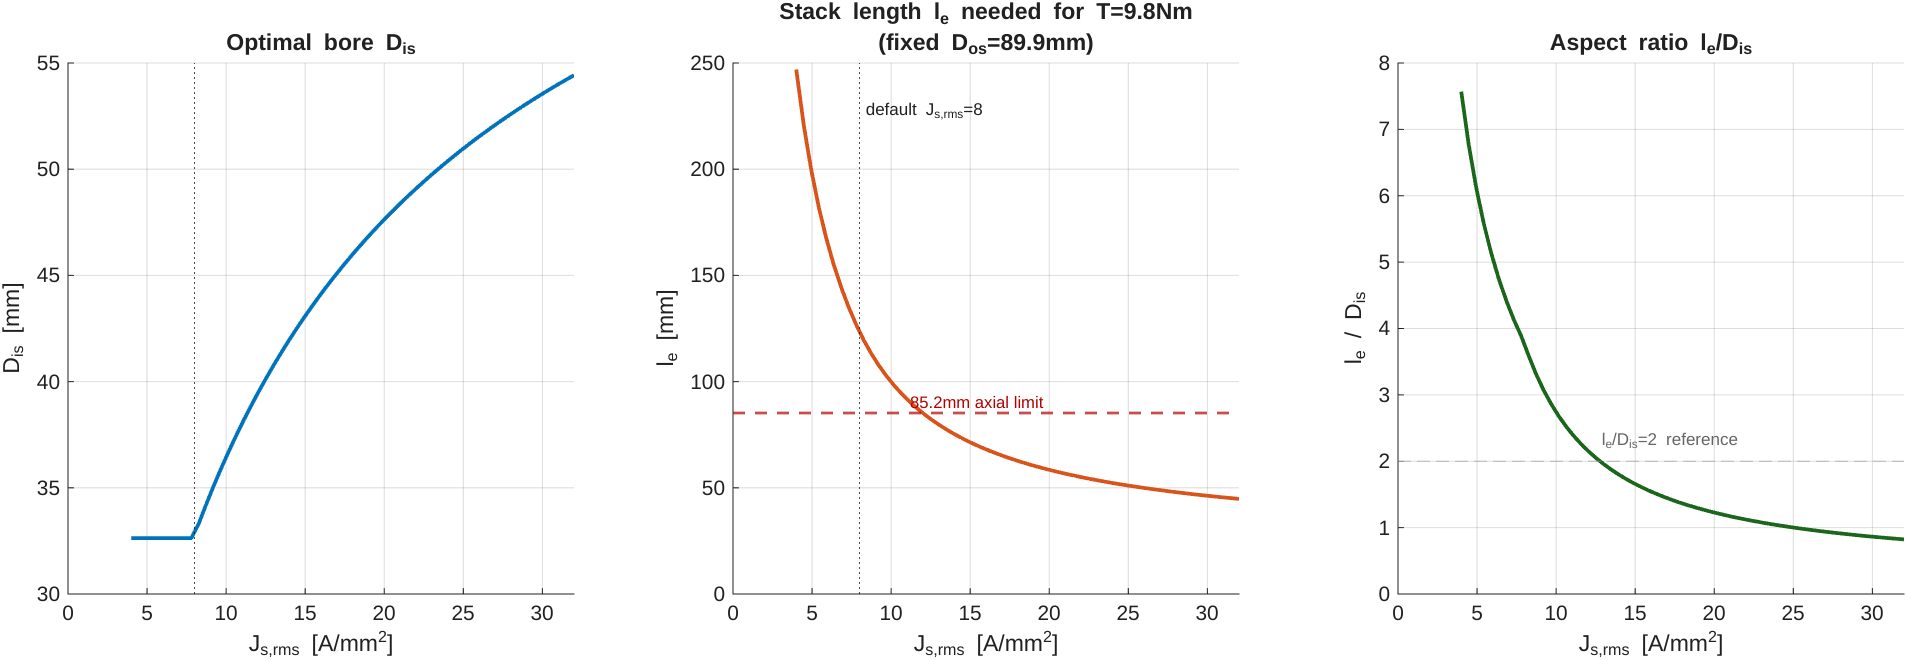
\includegraphics[width=0.9\textwidth]{figures/d3l_current_density_sensitivity.png}
\caption{Sensitivity of the Formula 2 to the current density $J_{s}$. Raising it to $\approx$12\,A/mm$^2$ brings $l_e$ down to our 85.2\,mm target.}
\label{fig:d3l_current_density_sensitivity}
\end{figure*}
\begin{table*}[!t]
\centering
\caption{Formula 1 vs. Formula 2 dimensions.}
\label{tab:formula1_vs_formula2}
\begin{tabular}{@{}lccc@{}}
\toprule
 & Formula 1 & Formula 2 ($J_{s,rms}=8\,\text{A/mm}^2$) & Formula 2 ($J_{s,rms}=12\,\text{A/mm}^2$) \\
\midrule
$D_{is}$ & 52.15 mm & 32.8 mm & 39.46 mm \\
$l_e$ & 32.77 mm & 123.5 mm & 85.2 mm \\
$l_e/D_{is}$ & 0.628 & 3.8 & 2.16 \\
\bottomrule
\end{tabular}
\end{table*}

\begin{figure*}[!t]
\centering
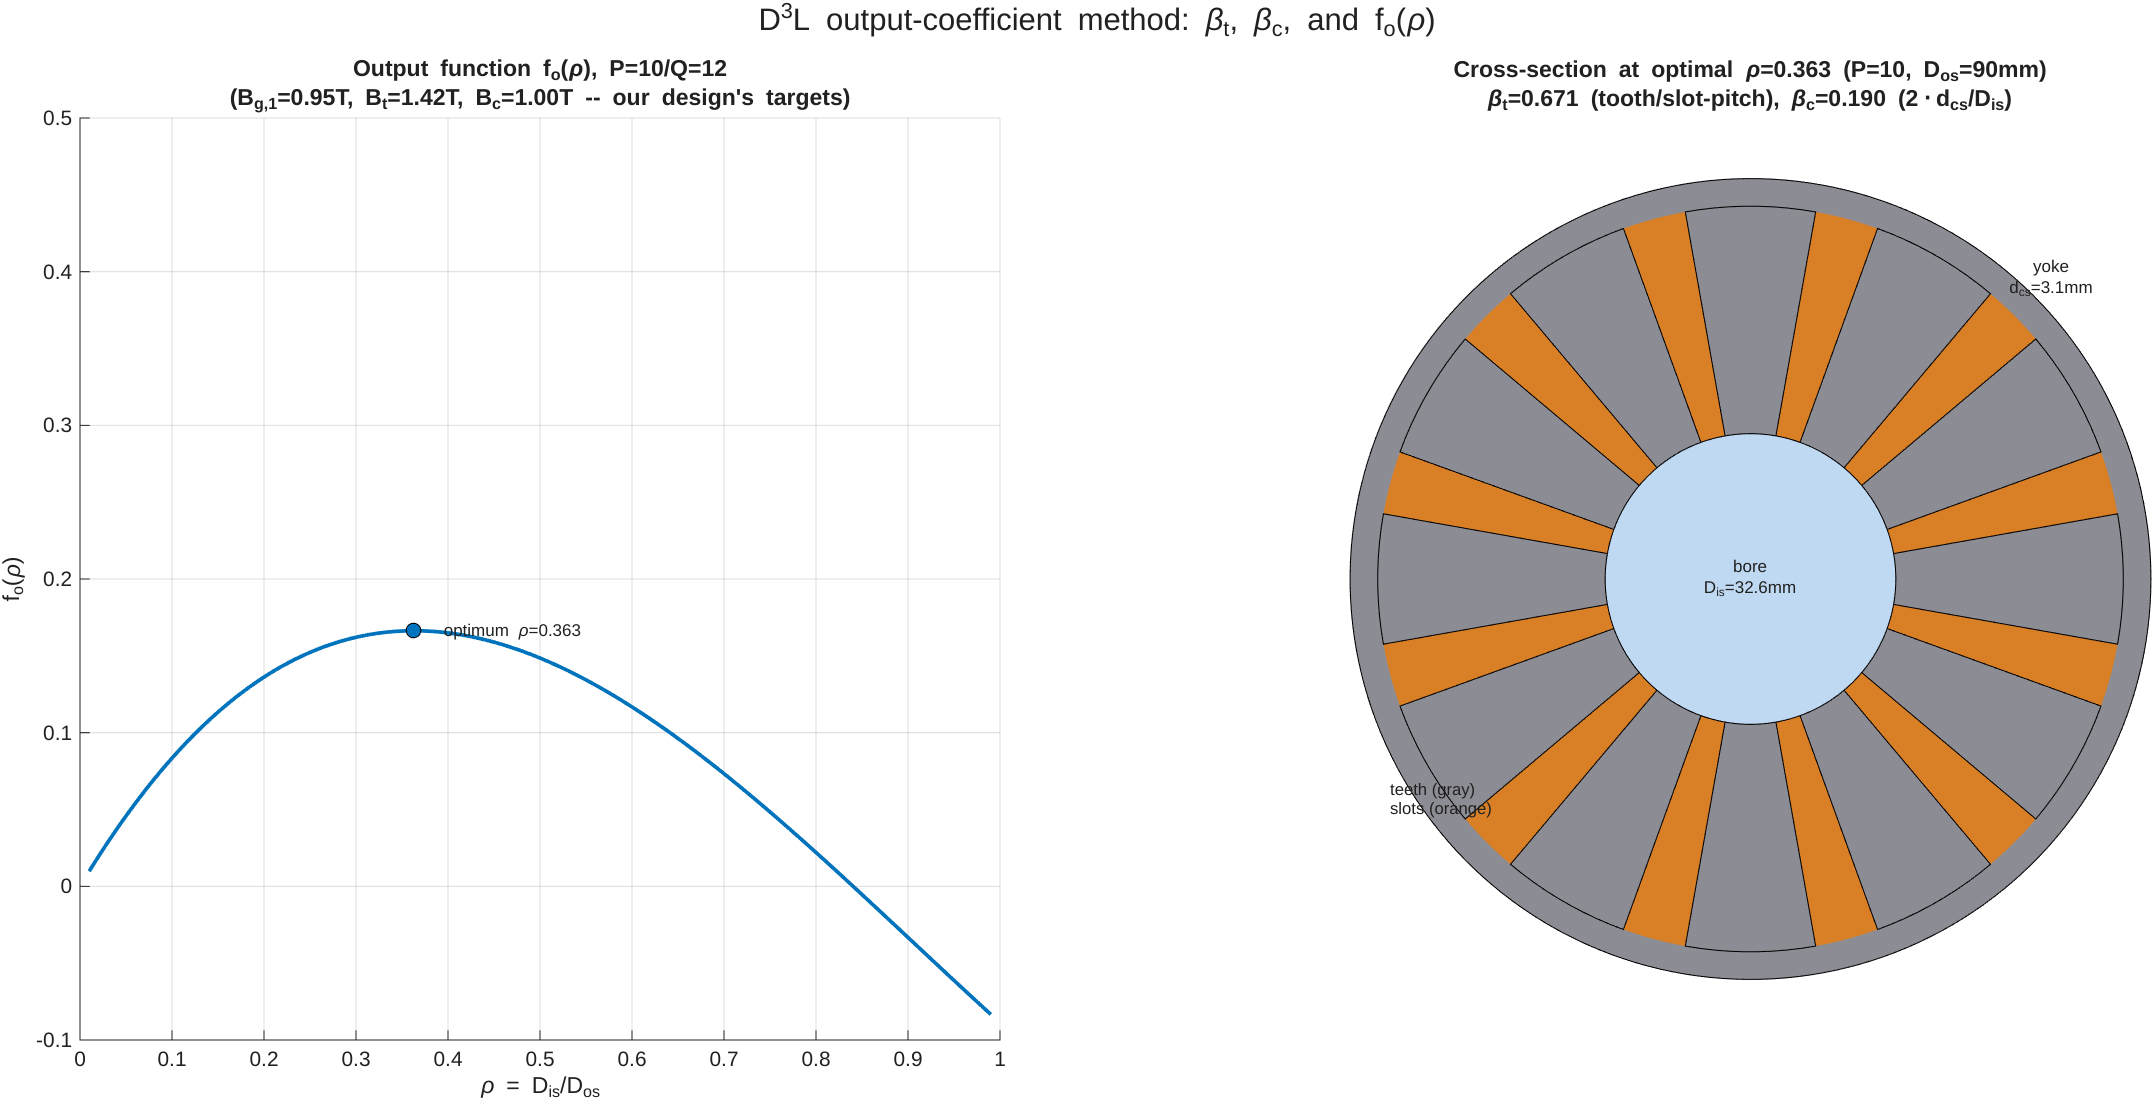
\includegraphics[width=0.9\textwidth]{figures/d3l_output_function.png}
\caption{Left: Optimum dimeter ratio optimum. Right: cross-section actual dimensions at optimal ratio.}
\label{fig:d3l_output_function}
\end{figure*}
Formula 2's bore (32.8\,mm) comes out noticeably smaller than Formula 1's 52.15\,mm. The two land on different rotor shapes as a result: Formula 1's $\lambda=2.0$ choice gives a fairly squat $l_e/D_{is}=0.628$, while Formula 2 independently derives a much longer, thinner $l_e/D_{is}\approx3.8$.
% TODO: Force a page break here.


\subsubsection{Magnet Material Selection}
\label{sec:magnet_material}
The choice of permanent magnet material sets the remanent flux density $B_r$ that feeds every downstream calculation, from Formula 1's magnetic shear stress $\sigma_m$ to the flux-linkage target below and Ricca's saturation model (\sectionname~\ref{sec:ricca_methodology}), so it needs to be pinned down before those. We select \textbf{sintered NdFeB, grade N48} \cite{ACHMagnetsN48}: NdFeB gives the highest energy product of common magnet families, which this application needs for torque density within the fixed 95.9\,mm/110\,mm envelope, and N48 sits at a good remanence/cost balance; higher grades (N52, N54) push $B_r$ only marginally higher at a steeper cost and availability penalty for a first design iteration.
\\\textbf{Remanence at 20\textdegree{}C ($B_{r,20}$):} \textbf{1.37 T}, from the datasheet \cite{ACHMagnetsN48}; in line with N48's typical 1.37--1.42\,T remanence range, and the value used throughout this project's sizing pipeline.
\\\textbf{PM operating temperature ($T_{PM}$):} \textbf{140\textdegree{}C}, set by the existing 4\,l/min liquid cooling loop's expected margin above ambient plus $I^2R$/core losses reaching the rotor. Standard N48 (no suffix) is typically only rated to $\approx$80--100\textdegree{}C before accelerated, irreversible demagnetization risk; sustaining 140\textdegree{}C safely calls for a high-temperature-stable variant (N48SH or better, rated $\gtrsim$150\textdegree{}C), to be confirmed against the specific part ordered, an open item for the next design iteration.
\\\textbf{Temperature-corrected remanence ($B_r$):} using a typical reversible temperature coefficient $\alpha_{Br}=-0.10\,\%/\text{\textdegree{}C}$,
\begin{equation}
\label{eq:br_derating}
\begin{split}
B_r &= B_{r,20}\left[1+\frac{\alpha_{Br}}{100}(T_{PM}-20)\right] \\
&= 1.37\left[1-0.001(140-20)\right] \approx 1.21\,\text{T}
\end{split}
\end{equation}
This is the value the flux-linkage/saturation model actually sees.
\\\textbf{Recoil permeability ($\mu_{rec}$):} \textbf{1.05}, typical for sintered NdFeB, used in the reluctance/anisotropy terms of Ricca's model (\sectionname~\ref{sec:ricca_methodology}).

\subsubsection{Corner Speed and Required Flux Linkage}
\label{sec:corner_speed}
The point where torque begins to fall is defined as the Corner Speed ($\omega_{base}$), occurring when the motor's internal Back-Electromotive Force (Back-EMF) reaches the maximum voltage available from the inverter. This relationship is governed by:

\begin{equation}
\omega_{m,base} \approx \frac{V_{\text{phase,peak,max}}}{p\,\Psi_m}
\end{equation}

Where $V_{\text{phase,peak,max}}$ is the maximum achievable \emph{phase} fundamental peak voltage, $p$ is the number of pole pairs, and $\Psi_m$ is the permanent magnet flux linkage.

The currently used AMK inverter considers a maximum continuous modulation index of $M_i=0.917$, which limits the maximum fundamental phase voltage to:
\begin{equation}
    V_{\text{phase,peak,max}} = M_i \frac{V_{DC}}{\sqrt{3}} \approx 0.917 \times \frac{515}{\sqrt{3}} \approx 273\,\text{V}
\end{equation}
To trigger the torque fall at an earlier speed, we must increase $\Psi_m$ (e.g., by increasing stator turns or selecting higher remanence magnets), thereby reducing $\omega_{m,base}$.

\texttt{main.m} fixes $n_{max}$ directly at the inverter's full 1200\,Hz / 14,400\,rpm cap (\tablename~\ref{tab:current_motor_data}, \sectionname~\ref{sec:Inverter}) and derives the corner speed as a fraction below it, $n_{base}=0.85\,n_{max}\approx12{,}240\,\text{rpm}$. With $p=5$ this gives a mechanical speed of $\omega_{m,base}\approx 1282\,\text{rad/s}$. Using the available $V_{\text{phase,peak,max}}\approx 273\,\text{V}$ yields a required order-of-magnitude flux linkage of:
\begin{equation}
    \Psi_m \approx \frac{V_{\text{phase,peak,max}}}{p\,\omega_{m,base}} \approx \frac{273}{5 \cdot 1282} \approx 0.0426\,\text{Wb}
\end{equation}
Ricca's procedure (\sectionname~\ref{sec:ricca_methodology}) now converges for this design point and gives $\Psi_{PM1}=0.0176\,\text{Wb}$ (\texttt{IPMRotorSizer.PsiPM1\_Wb}), only $\approx$40\% of the $\Psi_m$ target above, even with the N48 magnet (Eq.~\ref{eq:br_derating}, $B_r\approx1.21\,\text{T}$ at 140\textdegree{}C). This tracks the no-load flux-density shortfall flagged in \sectionname~\ref{sec:ricca_methodology}: with $B_{g,1o}$ itself running low for this pole pitch, $\Psi_{PM1}$ falls short too, so at the current turns/magnet geometry the machine reaches its corner point later than the 12,240\,rpm targeted here.

\subsubsection{Ricca's Paper Methodology}
\label{sec:ricca_methodology}
Formulas 1 and 2 give a fast first-pass envelope ($D_{is}$, $le_e$) from generic shear-stress/output-coefficient assumptions, but neither captures the distinctive properties of a V-shape rotor: PM flux leaks through the rotor bridges, there is magnetic saturation cross-coupling between the $d$- and $q$-axes, and reluctance-torque ($L_q>L_d$) is possible. For that, we implement the full analytical procedure of Di Gerlando \& Ricca \cite{DiGerlandoRicca2022} (\texttt{IPMRotorSizer.m}), used throughout the remaining subsections of Part A.

The procedure consists of five stages, each corresponding to a section of the paper:
\begin{enumerate}
    \item \textbf{Rotor geometry} (Section IV, eqs. 8--18): bridges, magnet width/thickness, V-angle and pole-shoe dimensions from the stator bore and pole pitch (\sectionname~\ref{sec:rotor_geometry}).
    \item \textbf{No-load saturation model} (Section II and III, eqs. 3--7, 38--42): air-gap flux, Carter factor and bridge leakage, giving the no-load flux density $B_{g,1o}$ (\sectionname~\ref{sec:stage2_saturation}).
    \item \textbf{Torque sizing and reaction coefficients} (Section V, eqs. 57--64, 96--110): the alignment/reluctance torque split, its geometric reaction coefficients (\sectionname~\ref{sec:torque_sizing_reaction_coefficients}), and the optimal current phase advance (\sectionname~\ref{sec:saturation_phase_advance}).
    \item \textbf{Stator winding and core sizing} (Section VI, eqs. 65--94): slot count, conductor count/gauge, tooth/yoke dimensions from the corner-point EMF and current density (\sectionname~\ref{sec:stator_winding_sizing}).
    \item \textbf{Electrical parameters} (Section VII, eqs. 95--120): $L_d$, $L_q$, $\Psi_{PM}$ (\sectionname~\ref{sec:electrical_parameters}).
\end{enumerate}
Geometry feeds saturation, saturation feeds torque sizing, and torque sizing feeds stator sizing. \texttt{IPMRotorSizer.solve()} iterates all five stages to convergence.

The paper's headline result is that torque splits into an alignment (PM) term and an anisotropy (reluctance) term, both functions of the current phase advance $\gamma$ (Eq.~\ref{eq:ricca_torque_pu}), where $\Delta$ is the linear current density, $c_d$ and $\sigma_{an}$ are geometric reaction coefficients from Stage 3 (\sectionname~\ref{sec:torque_sizing_reaction_coefficients}), $\lambda_{is}$ is the specific unsaturated reaction permeance (\textbf{not} the stator leakage inductance), $k_w$ the winding factor ($=k_1=0.91$, Formula 2's design targets above), and $\eta_\phi$ and $\sigma_s$ the PM-flux and iron saturation factors from stage 2 ($\eta_\phi$ here is $\eta_{\phi M}(M_q)$, \sectionname~\ref{sec:saturation_phase_advance}, evaluated at the current operating point). Maximizing Eq.~\ref{eq:ricca_torque_pu} over $\gamma$ gives the optimal phase advance $\gamma_{opt}$ used in \sectionname~\ref{sec:saturation_phase_advance}.

\begin{equation}
\label{eq:ricca_torque_pu}
\begin{split}
f_T(\Delta,\gamma) = {}& \underbrace{\eta_{\phi}\cos\gamma}_{f_{T,al}} \\
&+ \underbrace{\frac{\sqrt{2}\pi}{6}\,\frac{c_d\lambda_{is}}{k_w B_{g,1o}}\,\Delta\left(\sigma_{an}\sigma_s-1\right)\sin(2\gamma)}_{f_{T,an}}
\end{split}
\end{equation}

\subsubsection{Stage 1: Rotor Geometry}
\label{sec:rotor_geometry}
\begin{figure}[!htbp]
    \centering
    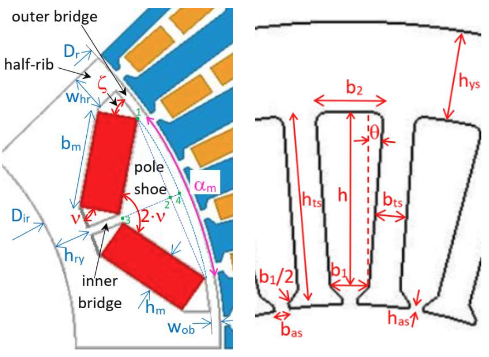
\includegraphics[width=0.85\columnwidth]{figures/IPM_motor_layout}
    \caption{V-Shape IPM Motor Layout}
    \label{fig:ipm_motor_layout}
\end{figure}
Stage 1 (\texttt{IPMRotorSizer.computeRotorGeometry\_}) turns the stator bore and five chosen shape ratios into the rotor's V-cavity dimensions. \textbf{We choose Formula 1's bore $D_{is}=52.15\,\text{mm}$} and air gap $g=1\,\text{mm}$, the rotor outer diameter, pole pitch  and stator slot pitch follow:
\begin{align*}
    D_r &= D_{is}-2g = 50.15\,\text{mm} \\
    \tau_r &= \frac{\pi D_r}{P} = 15.76\,\text{mm} \\
    \tau_s &= \pi D_{is}/N_s = 13.65\,\text{mm}
\end{align*}

Five quantities are chosen directly, each setting one part of the cavity shape ($\alpha_m$, $k_{rib}$, $t_m$, $\alpha_v$, and the $w_{ib}$/$w_{ob}$ bridge-width pair, five design choices across the six bullets below); the other two bullets ($w_{hr}$, $h_{ry}$) are derived from $k_{rib}$, not chosen independently, but are listed alongside them since they're needed immediately below:
\begin{itemize}[nosep]
    \item $\alpha_m=0.80$: magnet embrace ratio. Share of the pole pitch the pole shoe spans.
    \item $k_{rib}=0.1$: rib width as a fraction of the stator slot pitch ($\tau_s$).
    \item $w_{hr} = k_{rib}\,\tau_s = 1.365\,\text{mm}$ (\emph{derived}): half-rib width.
    \item $h_{ry} = 1.5\,w_{hr} = 2.05\,\text{mm}$ (\emph{derived}): rotor rib depth.
    \item $t_m=3\,\text{mm}$: Magnet segment height.
    \item $\alpha_v=78^\circ$: Magnet V-tilt angle.
    \item $w_{ib}=2.5\,\text{mm}$ and $w_{ob}=0.5\,\text{mm}$: bridge widths, sized by the structural bridge check of \sectionname~\ref{sec:bridge_sizing}.
\end{itemize}

These set the pole-shoe's tangential extension (eq.~\ref{eq:ps_ext}) and the inner bridge's radial length (eq.~\ref{eq:ib_len}):
\begin{equation}
    \label{eq:ps_ext}
    b_{ps} = \alpha_m\tau_r = 12.61\,\text{mm}
\end{equation}
\begin{equation}
    \label{eq:ib_len}
    h_{ib} = t_m\sin\alpha_v = 2.93\,\text{mm}
\end{equation}
A shared auxiliary length, the shoe's tangential half-width at the bridge corner, radius $D_r/2-w_{ob}$ (eq.~\ref{eq:d12}) then feeds both the pole-shoe's radial depth (eq.~\ref{eq:dps}) and the magnet width below (eq.~\ref{eq:wm}):
\begin{equation}
    \label{eq:d12}
    d_{12} = \left(\frac{D_r}{2}-w_{ob}\right)\sin\!\left(\alpha_m\frac{\pi}{P}\right) = 6.11\,\text{mm}
\end{equation}

\begin{equation}
    \label{eq:dps}
    \begin{split}
    d_{ps} = {}& \underbrace{\frac{d_{12}-w_{ib}/2}{\tan\alpha_v}}_{=\,1.03\,\text{mm}}
    + \underbrace{\left(\frac{D_r}{2}-w_{ob}\right) - \frac{d_{12}}{\tan(\alpha_m\pi/P)}}_{=\,0.77\,\text{mm}} \\
    &+ w_{ob} = 2.31\,\text{mm}
    \end{split}
\end{equation}

Eq.~\ref{eq:dps} gives the pole-shoe's radial depth. Eq.~\ref{eq:dir} checks the rotor bore, keeping the d-axis flux from short-circuiting across the shaft:
\begin{equation}
    \label{eq:dir}
    \begin{split}
    D_{ir} &= D_r - 2\,(d_{ps}+h_{ib}+h_{ry}) \\
    &= 50.15-2\,(2.31+2.93+2.05) = 35.58\,\text{mm}
    \end{split}
\end{equation}
Eq.~\ref{eq:wm} gives the magnet segment width:
\begin{equation}
    \label{eq:wm}
    w_m = \frac{d_{12}-w_{ib}/2}{\sin\alpha_v} = 4.97\,\text{mm}
\end{equation}

\subsubsection{Stage 2: No-load Saturation Model}
\label{sec:stage2_saturation}
Stage 2 (\texttt{IPMRotorSizer.computeSaturationModel\_}) turns the Stage 1 geometry and the stator slot opening into two results the rest of the procedure depends on: Carter's factor $k_C$ and the iron-saturation function $\sigma_{sM}(M_q)$ ($M_q$, and later $M_d$, the peak q-/d-axis reaction MMF, i.e.\ ampere-turns driven by the q-/d-axis stator current, $I_q$/$I_d$) that \sectionname~\ref{sec:saturation_phase_advance} evaluates at the corner-point MMF, and the no-load fundamental air-gap flux density $B_{g,1o}$ that anchors the specific-torque equation (Eq.~\ref{eq:specific_torque}) and everything after it.

\paragraph{Carter's factor.} We define the stator slot opening as $b_{as}=2\,\text{mm}$ (\texttt{spec.SlotOpening\_mm}). The Carter coefficient gives:
\begin{equation}
    \label{eq:carter_gamma}
    \gamma_C = \frac{(b_{as}/g)^2}{5+b_{as}/g} = \frac{2^2}{5+2} \approx 0.571
\end{equation}
\begin{equation}
    \label{eq:carter_factor}
    k_C = \frac{\tau_s}{\tau_s-\gamma_C\,g} = \frac{13.65}{13.65-0.571\times1} \approx 1.044
\end{equation}

\paragraph{No-load flux density.} At no load the PM alone drives the pole-shoe flux. The residual flux crossing the two magnet segments per pole, per unit stack length, is
\begin{equation}
    \label{eq:phi_pm}
    \phi_{PM} = B_r \cdot 2w_m = 1.206\times2\times4.97\times10^{-3} \approx 11.98\,\text{mWb/m}
\end{equation}
using the temperature-derated $B_r=1.206\,\text{T}$ (Eq.~\ref{eq:br_derating}) and the magnet width $w_m=4.97\,\text{mm}$ from Stage 1 (Eq.~\ref{eq:wm}). Part of this leaks locally through the inner/outer bridges instead of crossing the air gap; \texttt{IPMRotorSizer} models both bridges combined with a single constant leakage fraction, $\ell_{no\text{-}load}=16.6\%$ (\texttt{leakage\_no\_load}). As flagged in \sectionname~\ref{sec:ricca_methodology} and revisited in \sectionname~\ref{sec:sim_framework}, this constant is one of the report's open items: calibrated to the paper's larger pole pitch, it is documented to underestimate leakage by roughly 4--6$\times$ at this project's tighter 10-pole/12-slot geometry, and is the most likely single cause of the flux-linkage shortfall traced throughout \sectionname~\ref{sec:corner_speed}.

The specific flux actually reaching the pole shoe, and the resulting flux density averaged over the shoe's angular span $\alpha_m\tau_r$, follow as:
\begin{equation}
    \label{eq:phi_go}
    \begin{split}
    \phi_{go} &= \phi_{PM}\left(1-\ell_{no\text{-}load}\right)\alpha_m \\
    &= 11.98\times(1-0.166)\times0.80 \approx 7.996\,\text{mWb/m}
    \end{split}
\end{equation}
\begin{equation}
    \label{eq:b_go}
    B_{go} = \frac{\phi_{go}}{\alpha_m\tau_r} = \frac{7.996\times10^{-3}}{0.80\times15.76\times10^{-3}} \approx 0.634\,\text{T}
\end{equation}
where $\tau_r=15.76\,\text{mm}$ is the rotor pole pitch (\sectionname~\ref{sec:rotor_geometry}). $B_{go}$ is the flux density averaged over the pole-shoe arc; its fundamental Fourier component (used from now on) follows the standard width-$\alpha_m\pi$ square-wave factor:
\begin{equation}
    \label{eq:bg1o}
    B_{g,1o} = \frac{4}{\pi}\sin\!\left(\alpha_m\frac{\pi}{2}\right)B_{go} = \frac{4}{\pi}\sin(72^\circ)\times0.634 \approx 0.768\,\text{T}
\end{equation}
and, converting back to a specific flux for use alongside $\phi_{go}$ elsewhere in the procedure:
\begin{equation}
    \label{eq:phi_g1o}
    \phi_{g1o} = \frac{2}{\pi}B_{g,1o}\,\tau_r \approx 7.71\,\text{mWb/m}
\end{equation}
$B_{g,1o}=0.768\,\text{T}$ (\texttt{IPMRotorSizer.Bg1o\_T}) is the value quoted throughout the rest of Part A: the specific-torque equation (Eq.~\ref{eq:specific_torque}), the optimal phase advance search (\sectionname~\ref{sec:saturation_phase_advance}), and, downstream of the PM flux linkage $\Psi_{PM1}$, the corner-speed check of \sectionname~\ref{sec:corner_speed}.

\paragraph{Iron saturation function.}
In theory, as we increase the current $I_q$, the magnetic flux increases linearly along with the torque. In reality, iron saturates. We come up with an iron-saturation function $\sigma_{sM}(M_q)$, which is a penalty ranging from 1 (no saturation) to ~0.15 (full saturation). From \cite{DiGerlandoRicca2022} we extract M235-35A Extended permeability curve and convert that into an $H$-$B$ curve (\figurename~\ref{fig:bh_curve}).

\begin{figure}[!htbp]
\centering
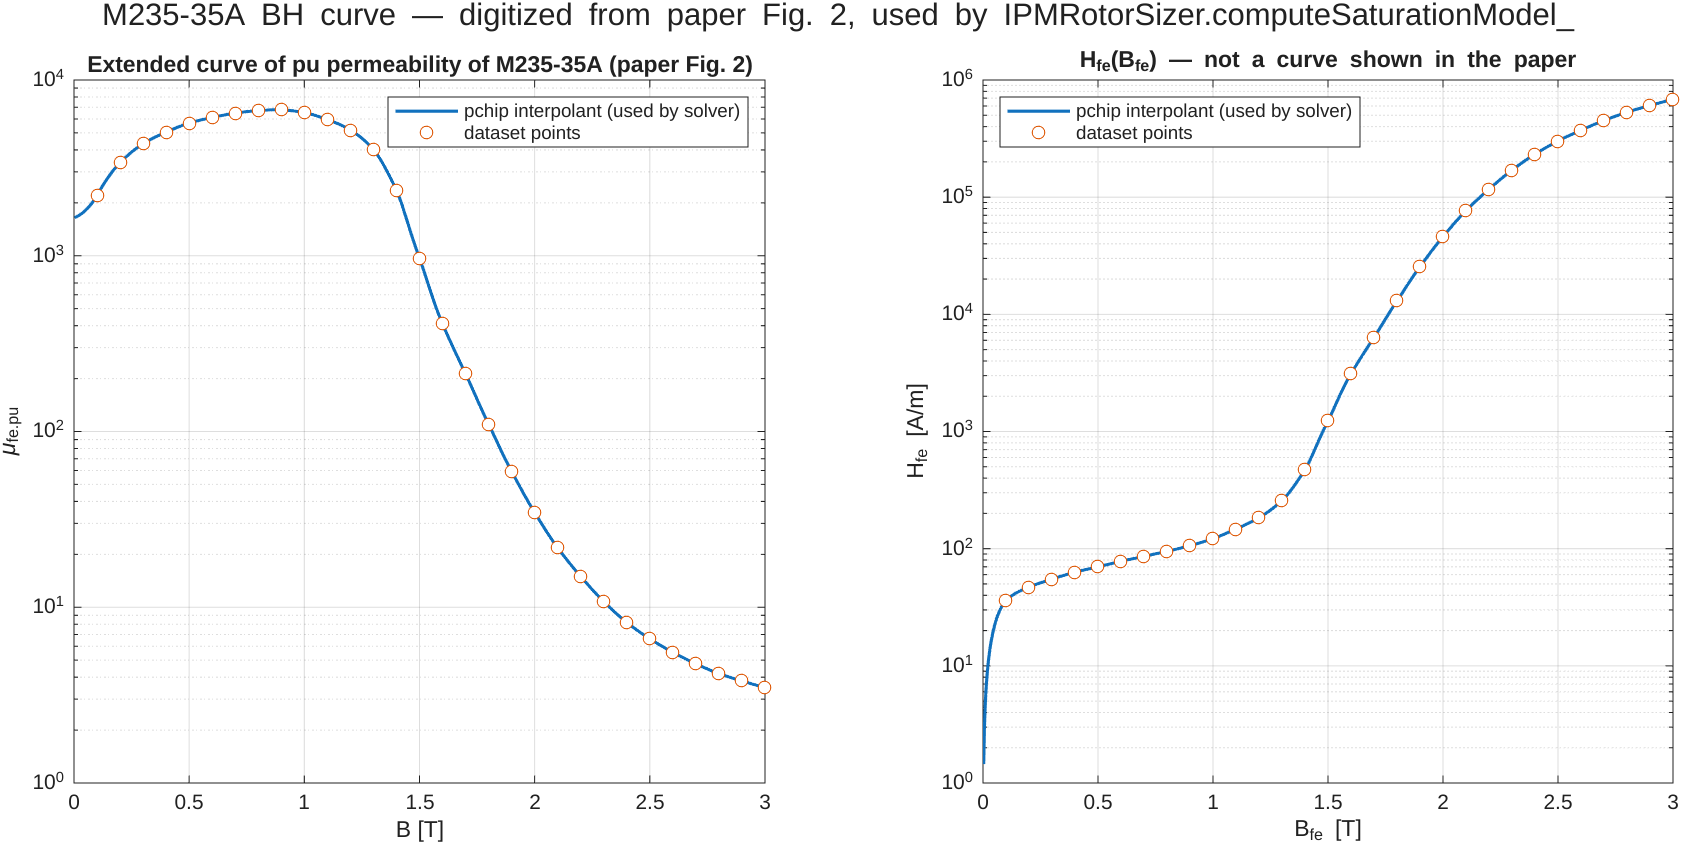
\includegraphics[width=\columnwidth]{figures/m235_35a_bh_curve.png}
\caption{M235-35A pu permeability and $H_{fe}(B)$ curve, the lattter used by the saturation model solver.}
\label{fig:bh_curve}
\end{figure}

The tooth flux density $B_{t}$ is solved implicitly from the air-gap flux density $B_{gI}$
\begin{equation}
    \label{eq:tooth_flux_implicit}
    B_t = \frac{B_{gI}}{\rho_{bt,s}\,k_{st}} - \frac{\mu_0 H_{fe}(B_t)}{k_{st}}\left(\frac{1}{\rho_{bt,s}}-1\right)
\end{equation}
where $B_{gI}$ is the peak air-gap flux density driven by the q-axis reaction MMF, $B_t$ the tooth flux density it induces, $\rho_{bt,s}$ the tooth-to-slot-pitch ratio, $\rho_{hte,g}$ the tooth-height-to-air-gap ratio, $\mu_0$ the permeability of free space, and $H_{fe}(\cdot)$ the BH-curve interpolant of \figurename~\ref{fig:bh_curve}. $B_t$ shows up on both sides here; once linearly, once inside the nonlinear $H_{fe}(\cdot)$ interpolant built from the BH curve (\figurename~\ref{fig:bh_curve}), so there's no closed-form solution. \texttt{computeSaturationModel\_} instead root-finds it (\texttt{fzero}) on a grid of $B_{gI}$ values and caches the result as a pchip interpolant $B_t(B_{gI})$, so the rest of the solve just looks it up instead of re-solving Eq.~\ref{eq:tooth_flux_implicit} on every call. This sets the saturation ratio
\begin{equation*}
\rho_{sat}(B_{gI})=1+H_{fe}(B_t)\,\rho_{hte,g}/(B_{gI}/\mu_0/k_C)
\end{equation*}
and the peak MMF needed to drive it,
\begin{equation*}
M_I(B_{gI})=B_{gI}\,g\,k_C\,\rho_{sat}/\mu_0
\end{equation*}
Inverting $M_I(B_{gI})$ for a given q-axis MMF $M_q$ gives $\sigma_{sM}(M_q)=B_p(M_q)\,g\,k_C/(\mu_0 M_q)$, plotted in \figurename~\ref{fig:saturation_factor}. The geometric ratios feeding this, $\rho_{bt,s}=b_{ts}/\tau_s$ and $\rho_{hte,g}=h_{te}/g$ (eqs. 86, 91), can't be pinned down here, but not both for the same reason. $b_{ts}$ (eq. 85: $b_{ts}=(B_{g,1o}/B_{ts})\tau_s/k_{st}$) only needs $B_{g,1o}$, already fixed above independently of everything in this loop, plus the fixed target $B_{ts}$ and the fixed $\tau_s$, $k_{st}$, so $\rho_{bt,s}$ isn't actually circular, it's just not sized until Stage 4 runs. $h_{te}$ is the genuinely circular one: it comes out of Stage 4's slot sizing, which needs the phase current and stack length $l_e$ that Stage 3 derives from $\sigma_{sM}(M_{q,c})$, i.e.\ from this very $\rho_{bt,s}$/$\rho_{hte,g}$ pair. \texttt{solve()} closes that loop by treating both, plus $c_d$ and $\sigma_{an}$ (\sectionname~\ref{sec:torque_sizing_reaction_coefficients}, circular by construction there), as its 4 iterative parameters: seeded at the paper's own Table~I values ($\rho_{bt,s}=0.704$, $\rho_{hte,g}=52.4$), re-derived by Stage 4 at the end of every outer-loop pass, and fed back into Stage 2 on the next. For this design the system reaches its fixed point in a single substantive pass ($\rho_{bt,s}\approx0.560$, $\rho_{hte,g}\approx32.0$); \texttt{Iterations}=2 just because the second pass is needed to confirm nothing moves further. Stage 2 itself only needs $\sigma_{sM}$ at $M_q=0$, where it is unsaturated by definition ($\sigma_{sM}\to1$), which is why the no-load flux above was derived independently, straight from the PM's own magnetic circuit, rather than by evaluating this function at zero.

\subsubsection{Rotor Bridge Sizing and Structural Integrity}
\label{sec:bridge_sizing}
The structural integrity of the IPM rotor is heavily dependent on the sizing of the inner ($w_{ib}$) and outer ($w_{ob}$) iron bridges. In this project the operating cap is $n_{max}=14{,}400\,\text{rpm}$ (\tablename~\ref{tab:motor_design_data}, \sectionname~\ref{sec:corner_speed}), and the bridge stress check is performed at this speed.
Electromagnetically, these bridges must be as thin as possible to minimize permanent magnet (PM) flux leakage. Mechanically, they must withstand the centrifugal forces exerted by the PM segments and the iron pole shoe.

Following the analytical model, the outer bridge is fixed to a minimum practical manufacturing thickness. In the current COMSOL/FEMM iteration this is set to $w_{ob}=0.5\,\text{mm}$ (\tablename~\ref{tab:params_defined}), while the inner bridge is sized to sustain the primary centrifugal load.

The maximum angular velocity for a mechanical speed $n_{max}$ is:
\begin{equation}
    \Omega_{max} = \frac{2\pi n_{max}}{60}
\end{equation}
For $n_{max}=14{,}400\,\text{rpm}$, $\Omega_{max}\approx 1508\,\text{rad/s}$.

The specific maximum centrifugal force ($f_{max}$) is calculated based on the mass of the pole shoe and magnets ($m_{1p}$) at average radius ($R_{av}$):

\begin{equation}
    f_{max} = m_{1p} \cdot R_{av} \cdot \Omega_{max}^2
\end{equation}

As a first-order estimate, the magnet contribution to $m_{1p}$ can be computed from the present geometry (two magnets per pole) as:
\begin{equation}
    m_{pm,1p} \approx 2\,\rho_{pm}\,w_m\,t_m\,L
\end{equation}
where $\rho_{pm}$ is the magnet density, $w_m=4.97\,\text{mm}$ (derived, eq.~\ref{eq:wm}, \tablename~\ref{tab:params_calculated}), $t_m=3\,\text{mm}$, and $l_e$ is the active stack length.

The stress on the inner bridge is then evaluated against the lamination yield strength ($\sigma_{y,lam}=460\,\text{MPa}$, M235-35A's 0.2\% proof yield strength in the rolling direction, \texttt{MotorMaterials.sigma\_y\_lam}) using a stress concentration factor ($K_t$):
\begin{equation}
    \sigma_{ib} = K_t \cdot \frac{f_{max}}{w_{ib} \cdot k_{st}} \leq \sigma_{y,lam}
\end{equation}
At the converged design point (\texttt{rotorSizer.summary()}), this gives $f_{max}\approx12{,}168\,\text{N/m}$ and $\sigma_{ib}\approx8.33\,\text{MPa}$, only 1.8\% of $\sigma_{y,lam}$, i.e.\ comfortably safe (\texttt{IPMRotorSizer.BridgeSafe}\,=\,true) with the current $w_{ib}=2.5\,\text{mm}$ inner bridge.

\begin{figure}[!htbp]
\centering
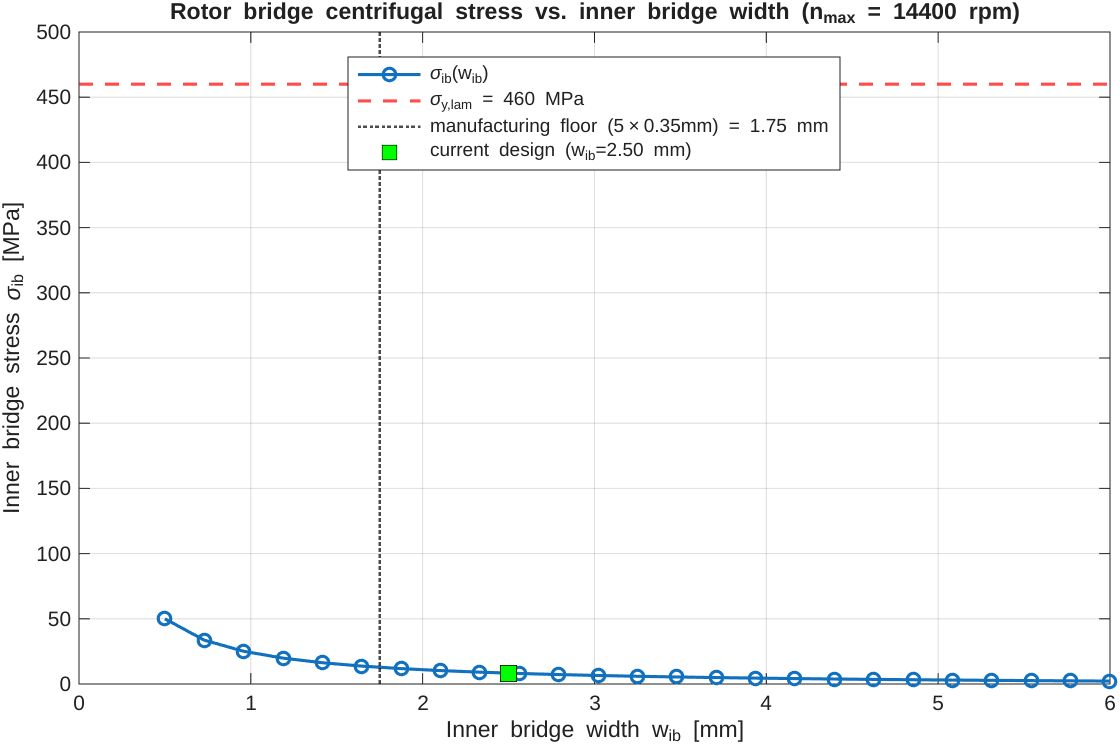
\includegraphics[width=\columnwidth]{figures/rotor_bridge_stress_sweep.png}
\caption{Inner bridge stress $\sigma_{ib}$ vs. bridge width $w_{ib}$ (\texttt{rotor\_bridge\_stress\_sweep.m}) at this project's own design point and $n_{max}=14{,}400\,\text{rpm}$, against the M235-35A yield line and the paper's $w_{ib}=5w_{ob}$ manufacturing-floor rule. The margin to yield stays large across the whole swept range; the bridge is not the constraining factor for this design.}
\label{fig:rotor_bridge_stress_sweep}
\end{figure}

\subsubsection{Stage 3: Torque Sizing and Reaction Coefficients}
\label{sec:torque_sizing_reaction_coefficients}
Eq.~\ref{eq:ricca_torque_pu}'s anisotropy term carries two purely geometric factors, $c_d$ and $\sigma_{an}=\sigma_{an,o}=c_q/c_d$, that this stage supplies (paper Section VII, eqs. 95--110; \texttt{IPMRotorSizer.\allowbreak computeElectricalParameters\_}). Physically, $c_d$ and $c_q$ are each the ratio of the actual fundamental reaction-field flux density, shaped by the pole shoe and blocked by the bridges (fully saturated by the PM leakage flux, hence treated as air), to the flux density an idealized \emph{isotropic} rotor of the same air gap would produce for the same reaction MMF:
\begin{equation}
\label{eq:bdis_bqis}
B_{d,is} = \frac{\mu_0 M_d}{k_C g}, \qquad B_{q,is} = \frac{\mu_0 M_q}{k_C g}
\end{equation}
Because the reaction MMFs $M_d$, $M_q$ enter every intermediate quantity linearly, they cancel out of the final ratios: $c_d$ and $c_q$ depend only on Stage 1's rotor geometry, not on the winding data or the operating current, consistent with the paper's own framing of the whole sizing procedure as independent of the winding data. The companion quantity $\lambda_{is}$, also needed by Eq.~\ref{eq:ricca_torque_pu}, is the specific (per-unit-length) unsaturated reaction permeance of an isotropic rotor of this same geometry (eq. 51):
\begin{equation}
\label{eq:lambda_is}
\lambda_{is} = \mu_0 k_w^2\,\frac{3}{\pi^2}\,\frac{\tau_r}{g\,k_C} = 4.78\,\mu\text{H/m}
\end{equation}
computed alongside $\gamma_{opt}$ in \texttt{computeTorqueSizing\_} (\sectionname~\ref{sec:saturation_phase_advance}).

Both reaction coefficients are extracted the same way: split the quarter-pole electrical angle $\theta_e\in[0,\pi/2]$ into the pole-shoe span $\theta_{ps}=\alpha_m\pi/2=72.0^\circ$ and, beyond it, the rib span out to
\begin{equation}
\label{eq:e_rib}
\theta_{e,rib} = \alpha_m\frac{\pi}{2} + p\,\frac{h_{ob}}{D_r/2} = 74.4^\circ
\end{equation}
where $h_{ob}=(\tau_r-2w_{hr}-b_{ps})/2=0.21\,\text{mm}$ (eq. 9, not previously shown in \sectionname~\ref{sec:rotor_geometry}) is the rotor-OD arc spanned by the outer bridge, small here because this design's wide pole shoe ($\alpha_m=0.80$) leaves little room between adjacent shoes, and $p=5$ pole pairs converts that mechanical arc into electrical radians. Beyond $\theta_{e,rib}$, out to $\pi/2$, the rotor is treated as isotropic (unslotted, no shoe).

\textbf{d-axis reaction (eqs. 96--106).} Within the shoe, the air-gap MVD is $M_d\cos\theta_e-U_{psd}$, where the pole-shoe potential $U_{psd}$ (unknown a priori) is fixed by a permeance balance at the shoe node: the flux the shoe pushes into the rotor interior, through the V-cavity permeance
\begin{equation}
\label{eq:lambda_ps_ir}
\Lambda_{ps,ir} = \mu_0\,l_e\,\frac{2w_m + t_m\cos\alpha_v + w_{ib}}{t_m} = 0.255\,\mu\text{H}
\end{equation}
(eq. 99), must equal the flux it delivers to the air gap through the shoe-facing permeance $\Lambda_g=\mu_0\alpha_m\tau_r l_e/(k_C g)=0.707\,\mu\text{H}$ (eq. 102). Solving that balance gives $U_{psd}$ in closed form (eq. 104):
\begin{equation}
\label{eq:upsd}
\frac{U_{psd}}{M_d} = \frac{\sin\theta_{ps}/\theta_{ps}}{1+\Lambda_{ps,ir}/\Lambda_g} = \frac{0.757}{1+0.361} = 0.556
\end{equation}
so over half of the shoe's reaction MVD is absorbed internally by the V-cavity rather than reaching the air gap, which is the mechanism that pulls $c_d$ well below 1. With $b_d(\theta_e)$ zero across the (fully saturated) rib and equal to the isotropic value $B_{d,is}\cos\theta_e$ beyond it, its fundamental component is now fully determined; the paper leaves $B_{d1}=\frac{4}{\pi}\int_0^{\pi/2}b_d(\theta_e)\cos\theta_e\,d\theta_e$ (eq. 105) as an integral to be evaluated numerically (a MathCad artifact; its own worked example just reports the resulting $c_d=0.201$, not a closed form). \texttt{IPMRotorSizer.m} instead evaluates it analytically, splitting the integral at $\theta_{ps}$ and $\theta_{e,rib}$ (Eq.~\ref{eq:cd_closed_form}).

\begin{figure*}[!t]
\normalsize
\begin{equation}
\label{eq:cd_closed_form}
c_d = \frac{B_{d1}}{B_{d,is}} = \frac{4}{\pi}\left[\underbrace{\frac{\theta_{ps}}{2}+\frac{\sin2\theta_{ps}}{4}-\frac{U_{psd}}{M_d}\sin\theta_{ps}}_{\text{shoe},\ [0,\,\theta_{ps}]} \;+\; \underbrace{\frac{\pi}{4}-\frac{\theta_{e,rib}}{2}-\frac{\sin2\theta_{e,rib}}{4}}_{\text{isotropic},\ [\theta_{e,rib},\,\pi/2]}\right] = 0.322 \quad\text{(eq. 106)}
\end{equation}
\begin{equation}
\label{eq:cq_closed_form}
c_q = \frac{B_{q1}}{B_{q,is}} = \frac{4}{\pi}\left[\underbrace{\frac{\theta_{ps}}{2}-\frac{\sin2\theta_{ps}}{4}}_{\text{shoe}} \;+\; \underbrace{\frac{\pi}{4}-\frac{\theta_{e,rib}}{2}+\frac{\sin2\theta_{e,rib}}{4}}_{\text{isotropic}}\right] = 0.951 \quad\text{(eq. 109)}
\end{equation}
\hrulefill
\vspace*{4pt}
\end{figure*}

\textbf{q-axis reaction (eqs. 107--110).} The q-axis case has no unknown potential to solve for: $b_q(\theta_e)=B_{q,is}\sin\theta_e$ holds across both the shoe and isotropic zones, zero across the rib as before (eq. 107). Its fundamental, $B_{q1}=\frac{4}{\pi}\int_0^{\pi/2}b_q(\theta_e)\sin\theta_e\,d\theta_e$ (eq. 108), therefore reduces to a similar closed form without the $U_{psd}$ term (Eq.~\ref{eq:cq_closed_form}), and the unsaturated anisotropy ratio used directly in Eq.~\ref{eq:ricca_torque_pu} follows:
\begin{equation}
\label{eq:sigma_an}
\sigma_{an} = \sigma_{an,o} = \frac{c_q}{c_d} = \frac{0.951}{0.322} \approx 2.95 \quad\text{(eq. 110)}
\end{equation}

With $c_d$, $\sigma_{an}$, and $\lambda_{is}$ fixed by geometry alone, that is everything Eq.~\ref{eq:ricca_torque_pu} needs from the reaction side; combining them with Stage 2's saturation factors ($\eta_\phi$, $\sigma_s$) to actually maximize $f_T$ over $\gamma$ and size the stack length is carried out next, in \sectionname~\ref{sec:saturation_phase_advance}. One subtlety worth flagging: because \texttt{computeTorqueSizing\_} (which evaluates $\gamma_{opt}$) runs \emph{before} \texttt{computeElectricalParameters\_} within a given pass of \texttt{solve()}, the $c_d$/$\sigma_{an}$ values it actually uses are the \emph{previous} iteration's converged result, seeded from the paper's own Table I defaults ($c_d=0.201$, $\sigma_{an,o}=4.11$) on the very first pass, which is itself part of why the five-stage loop needs more than one iteration to begin with (\sectionname~\ref{sec:ricca_methodology}); for this design point, \texttt{IPMRotorSizer.solve()} converges in 2 iterations.

\subsubsection{Magnetic Saturation and Optimal Phase Advance}
\label{sec:saturation_phase_advance}
Due to the highly saturated nature of the V-shape IPM design at the peak 107 A inverter limit, the d-q axis inductances cannot be treated as constant. The procedure utilizes a q-axis saturation model ($\sigma_{sM}$) and a PM flux cross-coupling saturation factor ($\eta_{\phi M}$) to account for the reduction of fundamental PM flux under heavy q-axis reaction current ($M_{pq}$).

The total electromagnetic torque is expressed as the sum of the alignment and anisotropy components:
\begin{equation}
    T(\Delta, \gamma) = T_{al}(\Delta, \gamma) + T_{an}(\Delta, \gamma)
\end{equation}

To maximize torque output within the current limit, the optimal phase advance angle ($\gamma_{opt}$) is dynamically calculated as a function of the linear current density ($\Delta$). This analytical $\gamma_{opt}$ provides the initial current angle for the FEA magnetostatic spatial sweep, ensuring the COMSOL model evaluates the motor at its Maximum Torque Per Ampere (MTPA) operating point.

Both the M235-35A BH curve and the resulting saturation factor $\sigma_{sM}(M_q)$ that feed this stage were validated against the reference paper's own Fig. 2/Fig. 3 at its worked-example design point (\sectionname~\ref{sec:ricca_methodology}), not this project's much smaller machine, and are shown here for that reason.
\begin{figure}[!htbp]
\centering
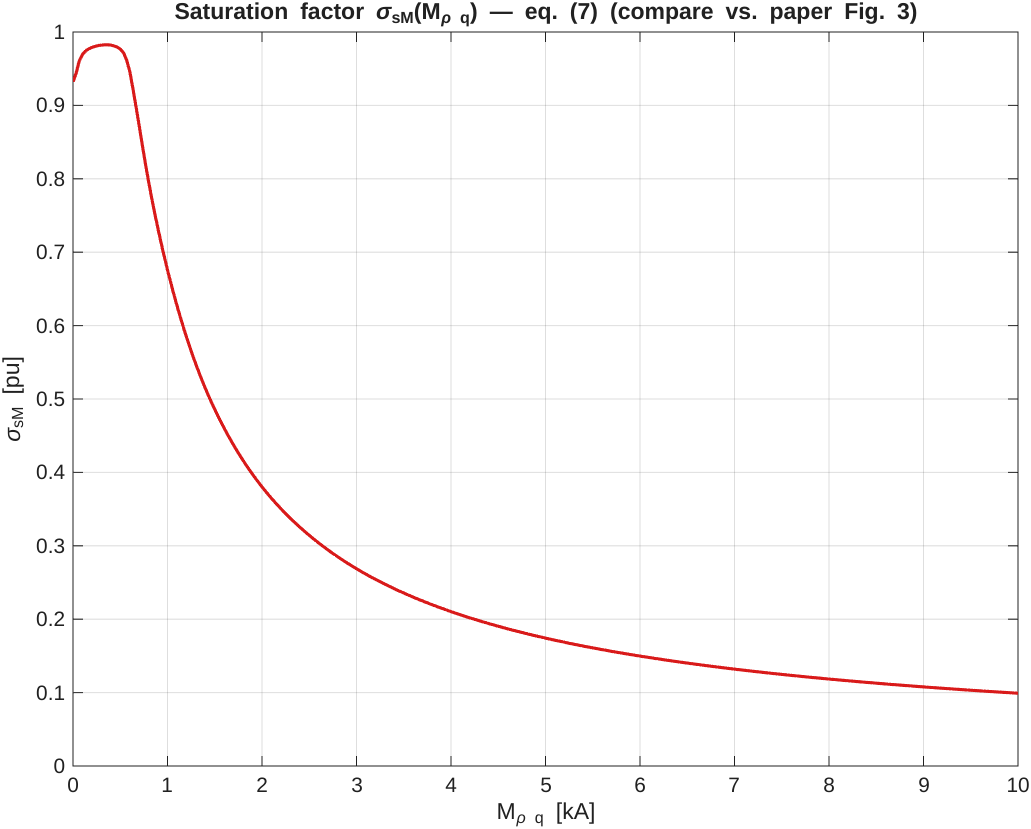
\includegraphics[width=0.8\columnwidth]{figures/saturation_factor_sigma_sM.png}
\caption{q-axis saturation factor $\sigma_{sM}(M_q)$ (eq. 7), eye-comparable against the paper's own Fig. 3.}
\label{fig:saturation_factor}
\end{figure}

Numerically maximizing Eq.~\ref{eq:ricca_torque_pu} over $\gamma$ at this design's operating point ($B_{g,1o}=0.77\,\text{T}$ from stage 2, \sectionname~\ref{sec:stage2_saturation}, $\Delta=90{,}000\,\text{A/m}$ RMS linear current density (\texttt{spec.LinearCurrentDensity\_Am}), $D_{is}=52.15\,\text{mm}$) gives the optimal phase advance $\gamma_{opt}=23.8^\circ$ and, evaluating the same equation there, the per-unit torque $f_{T,c}=1.107$. These convert to a specific torque (torque per unit stack length) and, dividing the target torque by it, the stack length:
\begin{equation}
    \label{eq:specific_torque}
    \begin{split}
    T_\ell &= f_{T,c}\cdot\frac{\pi k_w}{2\sqrt2}B_{g,1o}\Delta D_{is}^2 \\
    &= 1.107\times\frac{\pi\times0.91}{2\sqrt2}\times0.77\times90{,}000\times0.05215^2 \\
    &\approx 210.5\,\text{Nm/m}
    \end{split}
\end{equation}
\begin{equation}
    \label{eq:stack_length}
    l_e = \frac{T_{nom}}{T_\ell} = \frac{9.8}{210.5} \approx 46.6\,\text{mm}
\end{equation}

The same converged design point also fixes the phase current the rest of Part A and the FEM pipeline use. With $I_d=0$ (no field weakening at the corner/base torque point) and the converged $\Psi_{PM1}=0.0176\,\text{Wb}$ (\sectionname~\ref{sec:corner_speed}), the $I_q$ needed to produce the rated torque, and the resulting peak phase current, are:
\begin{equation}
    \label{eq:iq_current}
    \begin{aligned}
    I_q &= \frac{T_{nom}}{1.5\cdot(P/2)\cdot\Psi_{PM1}} = \frac{9.8}{1.5\times5\times0.0176} \approx 74.2\,\text{A}, \\
    I_{pk} &= \sqrt{I_d^2+I_q^2}=I_q\approx74.2\,\text{A}
    \end{aligned}
\end{equation}
This $I_{pk}=74.2\,\text{A}$ is a different quantity from the $I_{peak}\approx75.8\,\text{A}$ of \sectionname~\ref{sec:part_b_fea}: that one is an independent sanity check against the peak-\emph{power} requirement's assumed efficiency/power-factor, while $I_{pk}$ here is the actual current this specific converged rotor design needs to hit its rated \emph{torque}, given its real (flux-linkage-limited) $\Psi_{PM1}$; it is what actually gets pushed to the FEM (\tablename~\ref{tab:params_pushed}). Both stay comfortably under the 107\,A inverter limit.

\subsubsection{Stage 4: Stator Winding and Core Sizing}
\label{sec:stator_winding_sizing}
With the corner-point flux and current-density targets fixed, this stage sizes the winding turns, wire gauge, and stator tooth/slot/yoke dimensions (paper Section VI, eqs. 65--94; \texttt{IPMRotorSizer.\allowbreak computeStatorWindingSizing\_}), the source of every stator-side number already quoted in \tablename~\ref{tab:params_calculated}, not previously derived.

The fundamental pole flux at the corner point, and the EMF per conductor it induces, follow from Stage 2's no-load flux $\phi_{g1o}=7.71\,\text{mWb/m}$ and Stage 3's $\eta_{\phi,c}=0.983$ ($\eta_{\phi M}(M_q)$, \sectionname~\ref{sec:saturation_phase_advance}, evaluated at the corner-point MMF $M_{q,c}$; the ``$,c$'' subscript marks this operating-point value throughout Stage 4/5, same convention as $\sigma_{sM}$'s corner-point value $\sigma_{s,c}$), at the corner frequency $f_c=1020\,\text{Hz}$:
\begin{equation}
\label{eq:phi_g1c}
\begin{aligned}
\Phi_{g1c} &= \eta_{\phi,c}\,\phi_{g1o}\,l_e = 0.353\,\text{mWb}, \\
E_{cc} &= \frac{\pi}{\sqrt2}f_c\,\Phi_{g1c} = 0.80\,\text{V} \quad\text{(eqs. 65--66)}
\end{aligned}
\end{equation}
Targeting an EMF-over-voltage utilization $\rho_{EV}=0.65$ against the maximum inverter phase voltage $V_{invM}=0.95V_{dc}/(2\sqrt2)=173.0\,\text{V}$ (eq. 68, a different, more conservative voltage-limit model than the modulation-index one used in \sectionname~\ref{sec:corner_speed}; the two haven't been reconciled) gives the conductors in series, rounded through an even conductors-per-slot count:
\begin{equation}
\label{eq:conductors_series}
\begin{aligned}
U_{c,th} &= \frac{\rho_{EV}V_{invM}}{k_w E_{cc}} = 154.6, \\
u &= 2\,\text{round}\!\left(\tfrac12\,\frac{3U_{c,th}(P/2)}{N_s}\right) = 194, \\
U_c &= \frac{N_s u}{3(P/2)} = 155.2
\end{aligned}
\end{equation}
where $U_{c,th}$ is the unrounded target series-conductor count, $u$ the resulting (even, so each slot splits evenly across the two winding layers) conductors per slot, and $U_c$ the actual series-conductor count that rounding $u$ to an integer implies (eqs. 69, 72, 73). $U_c$ feeds Stage 5's inductances directly. Sizing the wire gauge from the current-density target $J_{s,rms}=8\,\text{A/mm}^2$, then the slot area from the copper fill factor $k_{Cu}=0.40$ (eqs. 76--84), fixes the tooth width and stator yoke height against the flux-density targets $B_{ts}=1.415\,\text{T}$, $B_{cs}=1.00\,\text{T}$:
\begin{equation}
\label{eq:tooth_yoke}
\begin{aligned}
b_{ts} &= \frac{B_{g,1o}}{B_{ts}}\frac{\tau_s}{k_{st}} = 7.64\,\text{mm} \quad\text{(eq. 85)}, \\
h_{sy} &= \frac{\phi_{g1o}}{2B_{cs}k_{st}} = 3.97\,\text{mm}
\end{aligned}
\end{equation}
using $\tau_s=13.65\,\text{mm}$ (\sectionname~\ref{sec:stage2_saturation}). Adding the resulting slot height ($h=22.9\,\text{mm}$, the closed-form root of a trapezoidal slot-area equation, eq. 89) and the slot-opening height $h_{as}=1.5\,\text{mm}$ (class default) to the bore gives the external stator diameter:
\begin{equation}
\label{eq:stator_od}
\begin{split}
D_{es} &= D_{is} + 2(h_{as}+h+h_{sy}) \\
&= 52.15 + 2(1.5+22.9+3.97) \approx 108.8\,\text{mm}
\end{split}
\end{equation}
matching \tablename~\ref{tab:params_calculated}'s stator diameter exactly (eq. 94). One open caveat: this same current-density/linear-current-density pairing also fixes a phase current $I_c=31.7\,\text{A}_{rms}$ (eq. 75) that is not what the rest of Part A or the FEM pipeline actually use: a third figure alongside the $I_{pk}=74.2\,\text{A}$ (Eq.~\ref{eq:iq_current}) and $I_{peak}\approx75.8\,\text{A}$ (\sectionname~\ref{sec:part_b_fea}) already flagged there, tracing to the same tension between the assumed linear current density $\Delta$ and the actual flux-linkage-limited torque point.

\subsubsection{Stage 5: Electrical Parameters}
\label{sec:electrical_parameters}
The last stage turns Stage 3's reaction coefficients and Stage 4's conductor count into the actual $d$/$q$ inductances and PM flux linkage (paper Section VII, eqs. 48, 52--56; \texttt{IPMRotorSizer.\allowbreak computeElectricalParameters\_}, the same method that computes $c_d$, $c_q$, \sectionname~\ref{sec:torque_sizing_reaction_coefficients}). The unsaturated reaction inductances follow directly from $\lambda_{is}$ (Eq.~\ref{eq:lambda_is}) and $U_c$ (Eq.~\ref{eq:conductors_series}):
\begin{equation}
\label{eq:ldo_lqo}
\begin{aligned}
L_{do} &= c_d\,\lambda_{is}\,\frac{U_c^2}{P}\,l_e = 0.172\,\text{mH}, \\
L_{qo} &= c_q\,\lambda_{is}\,\frac{U_c^2}{P}\,l_e = 0.509\,\text{mH} \quad\text{(eq. 52)}
\end{aligned}
\end{equation}
$L_d$ is taken equal to $L_{do}$ (eq. 54): the large equivalent d-axis air gap ($gk_C+t_m/\mu_{rec}$) keeps that axis close to linear, so its saturation is neglected. $L_q$ is not: it is scaled by Stage 3's saturation factor $\sigma_{s,c}=0.989$ at the operating point (eq. 55), and the resulting gap is exactly the reaction-inductance difference driving Eq.~\ref{eq:ricca_torque_pu}'s anisotropy term (eq. 56):
\begin{equation}
\label{eq:lq_final}
L_q = L_{qo}\,\sigma_{s,c} = 0.504\,\text{mH}, \qquad L_q - L_d = 0.331\,\text{mH}
\end{equation}
The PM flux linkage, already used without derivation in Eq.~\ref{eq:iq_current} and \sectionname~\ref{sec:corner_speed}, follows the same pattern (eq. 48):
\begin{equation}
\label{eq:psipm1}
\begin{split}
\Psi_{PM1} &= \frac{k_w U_c \phi_{g1o}\,\eta_{\phi,c}}{2\sqrt2}\,l_e \\
&= \frac{0.91\times155.2\times0.00771\times0.983}{2\sqrt2}\times0.04656 \\
&\approx 0.0176\,\text{Wb}
\end{split}
\end{equation}
Not computed by this pipeline: the true phase leakage inductance $L_\ell$ and AC winding resistance $R(f)$ (paper Section VII.C, eqs. 111--119), already flagged in passing at \sectionname~\ref{sec:torque_sizing_reaction_coefficients}'s $\lambda_{is}$ correction. With $L_d$, $L_q$, and $\Psi_{PM1}$ fixed, everything Part A's summary tables below actually draw on (rotor geometry, stack length, phase advance, stator core, and rated current) now traces back to a shown equation rather than an unexplained number.

The following table summarizes the first design objectives (\tablename~\ref{tab:motor_design_data}).

\begin{table*}[!t]
\centering
\footnotesize
\caption{New Design Objectives}
\label{tab:motor_design_data}
\begin{tabular}{@{}L{0.16\linewidth} p{0.06\linewidth} L{0.17\linewidth} L{0.53\linewidth}@{}}
\toprule
\textit{Parameter} & \textit{Symbol} & \textit{Value} & \textit{Engineering Justification} \\
\midrule
\textbf{Pole Number} & $P$ & 10 & Sized to maximize the AMK RACING KIT inverter frequency limit. \\
\textbf{Slot Number} & $N_s$ & 12 & Low cogging torque when combined with the 10 poles. \\
\textbf{Stack Length} & $l_e$ & 46.6 mm & Ricca's converged torque-sizing result (eq.~\ref{eq:stack_length}, \sectionname~\ref{sec:saturation_phase_advance}). \\
\textbf{Stator Outer Diameter} & $D_{es}$ & 108.8 mm & From Stage 4 (\sectionname~\ref{sec:stator_winding_sizing}), eq.~94. Not $D_{os}$; that symbol is reserved for the \emph{old} motor's 89.9\,mm stator OD (\tablename~\ref{tab:current_motor_data}). \\
\textbf{DC-link Voltage} & $V_{DC}$ & 515 V & Assumed tractive-system bus voltage (\sectionname~\ref{sec:Inverter}); within the AMK inverter's 500--600 V DC documented range. Same value as \tablename~\ref{tab:current_motor_data}: it is the one inverter, reused. \\
\textbf{Target Nominal Power} & $P_{nom}$ & $\approx$12.6 kW & $P_{nom}=T_{nom}\cdot\omega_{base}=9.8\,\text{Nm}\times1281.8\,\text{rad/s}$ at the corner speed. \\
\textbf{Target Peak Power} & $P_{peak}$ & 26 kW & Sized to maximize the inverter capacity (26 kVA/channel, the inverter's own \texttt{KW26} model designation). Not reconciled with Part B's current-limit check (\sectionname~\ref{sec:part_b_fea}), which instead uses the boundary requirement's 28\,kW directly (\tablename~\ref{tab:propulsion_motor_requirements}). \\
\textbf{Magnet Material} & $B_r$ & N48 NdFeB: 1.37 T (20\textdegree{}C) / 1.21 T (140\textdegree{}C) & Selected in Magnet Material Selection (\sectionname~\ref{sec:magnet_material}) for its remanence/cost balance; the temperature-corrected value is what Ricca's saturation model (\sectionname~\ref{sec:ricca_methodology}) actually uses. \\
\textbf{Required Flux Linkage} & $\Psi_m$ & $\approx$0.0426 Wb & From the corner-speed back-EMF constraint at $n_{base}=12{,}240\,\text{rpm}$ (\sectionname~\ref{sec:corner_speed}). \\
\textbf{Target Nominal Torque} & $T_{nom}$ & 9.8 Nm & Matches both (\tablename~\ref{tab:current_motor_data}) and (\tablename~\ref{tab:propulsion_motor_requirements}). \\
\textbf{Peak Torque} & $M_{clip}$ & 21.5 Nm & Boundary requirement (\tablename~\ref{tab:propulsion_motor_requirements}, 5\,s rating).\\
\textbf{Target Max Speed} & $n_{max}$ & 14,400 rpm & Set directly to the inverter's full 1200 Hz / 14,400 rpm cap (\tablename~\ref{tab:current_motor_data}, \sectionname~\ref{sec:Inverter}). \\
\textbf{Target Corner Speed} & $n_{base}$ & 12,240 rpm & Target $\approx$1.18 flux-weakening ratio (\sectionname~\ref{sec:corner_speed}). \\
\textbf{Rotor Topology} & n/a & IPM & Selected to achieve reluctance-torque contribution (Eq.~\ref{eq:ricca_torque_pu}). \\
\bottomrule
\end{tabular}
\end{table*}

For traceability, this section funnels the design pipeline through three views of the same design point: what we \textbf{define} directly (\tablename~\ref{tab:params_defined}), what the sizing chain then \textbf{calculates} from those choices (\tablename~\ref{tab:params_calculated}), and finally the subset of both that actually gets \textbf{pushed to COMSOL} (\tablename~\ref{tab:params_pushed}) as Global Parameters for the FEA model. \texttt{IPMRotorSizer.solve()} converges end-to-end for this design point (\texttt{main.m}: \texttt{AlphaM=0.80}, \texttt{Whr\_fraction=0.1}, \texttt{Hm\_mm=3}), so every value below is its actual solved output, not a placeholder. The stack length here ($l_e=46.6$\,mm, eq.~\ref{eq:stack_length}) is Ricca's own electromagnetically-driven result, distinct from Formula 1/2's Esson-rule estimates (\sectionname~\ref{sec:ricca_methodology} reconciliation discussion); the two sizing passes have not yet been cross-checked against each other.

\begin{table*}[!t]
\centering
\footnotesize
\caption{Design choices defined directly}
\label{tab:params_defined}
\begin{tabular}{@{}L{0.22\linewidth}p{0.08\linewidth}L{0.40\linewidth}L{0.22\linewidth}@{}}
\toprule
\textbf{Parameter} & \textbf{Symbol} & \textbf{MATLAB Variable} & \textbf{Value} \\
\midrule
Number of poles & $N_p$ & \texttt{spec.Poles} & 10 \\
Number of slots & $N_s$ & \texttt{spec.Slots} & 12 \\
Airgap & $g$ & \texttt{spec.Airgap\_mm} & 1 mm \\
Speed (operating cap) & $n_{max}$ & \texttt{spec.MaxSpeed\_rpm} & 14,400 rpm \\
Magnet height & $t_m$ & \texttt{rotorSizer.Hm\_mm} & 3 mm \\
V-angle & $\alpha_v$ & \texttt{rotorSizer.Vtilt\_deg} & 78$^\circ$\\
Outer bridge thickness & $w_{ob}$ & \texttt{rotorSizer.Wob\_mm} & 0.5 mm \\
\bottomrule
\end{tabular}
\end{table*}

\begin{table*}[!t]
\centering
\footnotesize
\caption{Sizing results calculated from the choices above}
\label{tab:params_calculated}
\begin{tabular}{@{}L{0.22\linewidth}p{0.08\linewidth}L{0.40\linewidth}L{0.22\linewidth}@{}}
\toprule
\textbf{Parameter} & \textbf{Symbol} & \textbf{MATLAB Variable} & \textbf{Value} \\
\midrule
Rotor diameter & $D_r$ & \texttt{rotorSizer.RotorOD\_mm} & 50.15 mm \\
Shaft diameter & $D_{ir}$ & \texttt{rotorSizer.RotorID\_mm} & 35.58 mm \\
Stator diameter & $D_{es}$ & \texttt{rotorSizer.StatorOD\_mm} & 108.8 mm \\
Stator yoke height & $h_{sy}$ & \texttt{rotorSizer.StatorYoke\-Height\_mm} & 3.97 mm \\
Stack length & $l_e$ & \texttt{rotorSizer.StackLength\_mm} & 46.6 mm \\
Corner speed & $n_{base}$ & \texttt{spec.CornerSpeed\_rpm} & 12,240 rpm \\
Phase current & $I_{pk}$ & \texttt{hypot(motorGeometry.Id\_A,\allowbreak\ motorGeometry.Iq\_A)} & 74.2 A (phase peak, eq.~\ref{eq:iq_current}) \\
Magnet width (slab) & $w_m$ & \texttt{rotorSizer.Bm\_mm} & 4.97 mm \\
\bottomrule
\end{tabular}
\end{table*}

\begin{table*}[!t]
\centering
\footnotesize
\caption{Values pushed to COMSOL as Global Parameters}
\label{tab:params_pushed}
\begin{tabular}{@{}L{0.20\linewidth}L{0.13\linewidth}L{0.13\linewidth}L{0.18\linewidth}L{0.20\linewidth}@{}}
\toprule
\textbf{Parameter} & \textbf{COMSOL Param} & \textbf{Value} & \textbf{Source} & \textbf{Pushed by} \\
\midrule
Number of poles & \texttt{Np} & 10 & \tablename~\ref{tab:params_defined} & \texttt{pushGeometry} \\
Number of slots & \texttt{Ns} & 12 & \tablename~\ref{tab:params_defined} & \texttt{pushGeometry} \\
Airgap & \texttt{airgap} & 1 mm & \tablename~\ref{tab:params_defined} & \texttt{pushGeometry} \\
Speed (structural sweep) & \texttt{w\_rot} & 14,400 rpm & \tablename~\ref{tab:params_defined} & \texttt{pushGeometry} \\
Rotor diameter & \texttt{d\_r} & 50.15 mm & \tablename~\ref{tab:params_calculated} & \texttt{pushGeometry} \\
Shaft diameter & \texttt{d\_s} & 35.58 mm & \tablename~\ref{tab:params_calculated} & \texttt{pushGeometry} \\
Stator yoke height & \texttt{h\_sy} & 3.97 mm & \tablename~\ref{tab:params_calculated} & \texttt{pushGeometry} \\
Stack length & \texttt{L} & 46.6 mm & \tablename~\ref{tab:params_calculated} & \texttt{pushGeometry} \\
Phase current (peak) & \texttt{Ipk} & 74.2 A & \tablename~\ref{tab:params_calculated} & \texttt{pushExcitation} \\
\bottomrule
\end{tabular}
\end{table*}

\section{Part B: Finite Element Analysis and Validation}
\label{sec:part_b_fea}
To validate the Part A results, a simulation loop has been established using a MATLAB interface (LiveLink for MATLAB, over Python, since the entire analytical sizing chain in \sectionname~\ref{sec:ricca_methodology} is already MATLAB, avoiding a second language boundary between sizing and simulation). The objective is to verify the results and make necessary adjustments to the design parameters, taking the simulation results as more accurate than the analytical model.

\subsection{Electromechanical Power Modeling}
Since the motor is not 100\% efficient, we represent the electrical input power ($P_{elec}$) relative to the mechanical shaft power ($P_{mech}$) through the overall efficiency ($\eta$).
\begin{equation}
    P_{elec} = \frac{P_{mech}}{\eta}
\end{equation}

The electrical power for a 3-phase system is defined as:
\begin{equation}
    P_{elec} = \frac{3}{2} V_{peak} I_{peak} \cos(\phi)
\end{equation}

Here, $V_{peak}$ and $I_{peak}$ refer to \emph{phase} sinusoidal peak quantities. Using SVPWM, a common approximation for the maximum achievable fundamental phase voltage is $V_{peak}\approx V_{dc}/\sqrt{3}$.

Rearranging for the current limit validation, and plugging in the peak power target $P_{mech}=28\,\text{kW}$, this project's DC-link voltage $V_{dc}=515\,\text{V}$, $\eta=0.92$ and $\cos(\phi)=0.90$:
\begin{equation}
\begin{split}
    I_{peak} &= \frac{2 \cdot P_{mech}}{\sqrt{3} \cdot V_{dc} \cdot \eta \cdot \cos(\phi)} \\
    &= \frac{2\times28\,\text{kW}}{\sqrt{3}\times515\,\text{V}\times0.92\times0.90} \approx 75.8\,\text{A}
\end{split}
\end{equation}

\subsection{Simulation Framework}
\label{sec:sim_framework}
In \texttt{main.m}, a single driver class, \textbf{\texttt{ComsolPrebuiltInterface}} (\texttt{RUN\_COMSOL\_PREBUILT}), takes the \texttt{MotorGeometry} built from the converged sizing results (\sectionname~\ref{sec:ricca_methodology}) and pushes the eight design values that actually change between design iterations (pole/slot count, air gap, stator yoke height, rotor diameter, shaft rotor-bore diameter, stack length, and the rotation speed the structural sweep runs at, $w_{rot}=n_{max}$) as Global Parameters into a pre-built COMSOL AC/DC Application-Library model, then rebuilds only the geometry sequence. Its read-only template (\texttt{interior\_\allowbreak pm\_\allowbreak motor\_\allowbreak stress\_\allowbreak analysis\_\allowbreak original.mph}) is never written to; results save to a separate output file. Pushing parameters into a template this way avoids the meshing/physics setup overhead of a from-scratch geometric redraw on every design iteration. Study results are cached by design point (\texttt{ComsolPrebuiltInterface.runStudyCached}, \texttt{COMSOL\_models/cache/}): re-running \texttt{main.m} at an unchanged design point reuses the previous $\approx$20-minute coupled EM/structural solve instead of repeating it, while a genuinely new design point still triggers a fresh solve automatically.

Exercising this pipeline end-to-end for the converged design point (\tablename~\ref{tab:params_pushed}) gives the results in \tablename~\ref{tab:fem_results}. The FEM-predicted average torque, $8.48\,\text{Nm}$, comes in $13.5\%$ below the $9.8\,\text{Nm}$ analytical target, consistent \emph{in direction} with the flux-linkage shortfall already flagged in \sectionname~\ref{sec:corner_speed}: since the converged $\Psi_{PM1}$ falls short of the target the analytical torque sizing assumes, that sizing is itself optimistic, and the FEM, seeing the true (lower) flux at the same pushed current ($I_{pk}=74.2\,\text{A}$, \tablename~\ref{tab:params_pushed}), produces correspondingly less torque. The two gaps aren't the same size, though: $\Psi_{PM1}$ is only $\approx$41\% of its $\Psi_m$ target (\sectionname~\ref{sec:corner_speed}), a much larger shortfall than 13.5\%, so this is a directional, not magnitude, cross-check; no FEM-side flux-linkage or back-EMF extraction exists yet (\texttt{ComsolPrebuiltInterface.resultsSummary} only reads torque, stress, and displacement) to test whether the two gaps actually reconcile quantitatively. Torque ripple is a modest $4.9\%$. The coupled structural solve puts peak von Mises stress at $63.0\,\text{MPa}$ ($13.7\%$ of $\sigma_{y,lam}=460\,\text{MPa}$, \sectionname~\ref{sec:bridge_sizing}) and peak displacement at $69\,\mu\text{m}$, both comfortably within margin. The FEM stress is notably higher than the analytical bridge-only check ($8.33\,\text{MPa}$, \sectionname~\ref{sec:bridge_sizing}): the FEM captures the full 2D stress field (geometric concentrations, electromagnetic force contributions) rather than just the idealized centrifugal-load bridge model, so this is expected and not a contradiction.

\begin{table}[!t]
\centering
\caption{Coupled EM/structural transient study results (\texttt{ComsolPrebuiltInterface.resultsSummary}), converged design point}
\label{tab:fem_results}
\begin{tabular}{@{}L{0.52\columnwidth}L{0.38\columnwidth}@{}}
\toprule
\textbf{Result} & \textbf{Value} \\
\midrule
Average axial torque (rmm.Tark\_1, Arkkio method) & 8.48 Nm \\
Torque ripple & 4.9\% \\
Peak von Mises stress & 63.0 MPa (13.7\% of $\sigma_{y,lam}$) \\
Peak displacement & 0.069 mm \\
\bottomrule
\end{tabular}
\end{table}

\begin{figure}[!htbp]
\centering
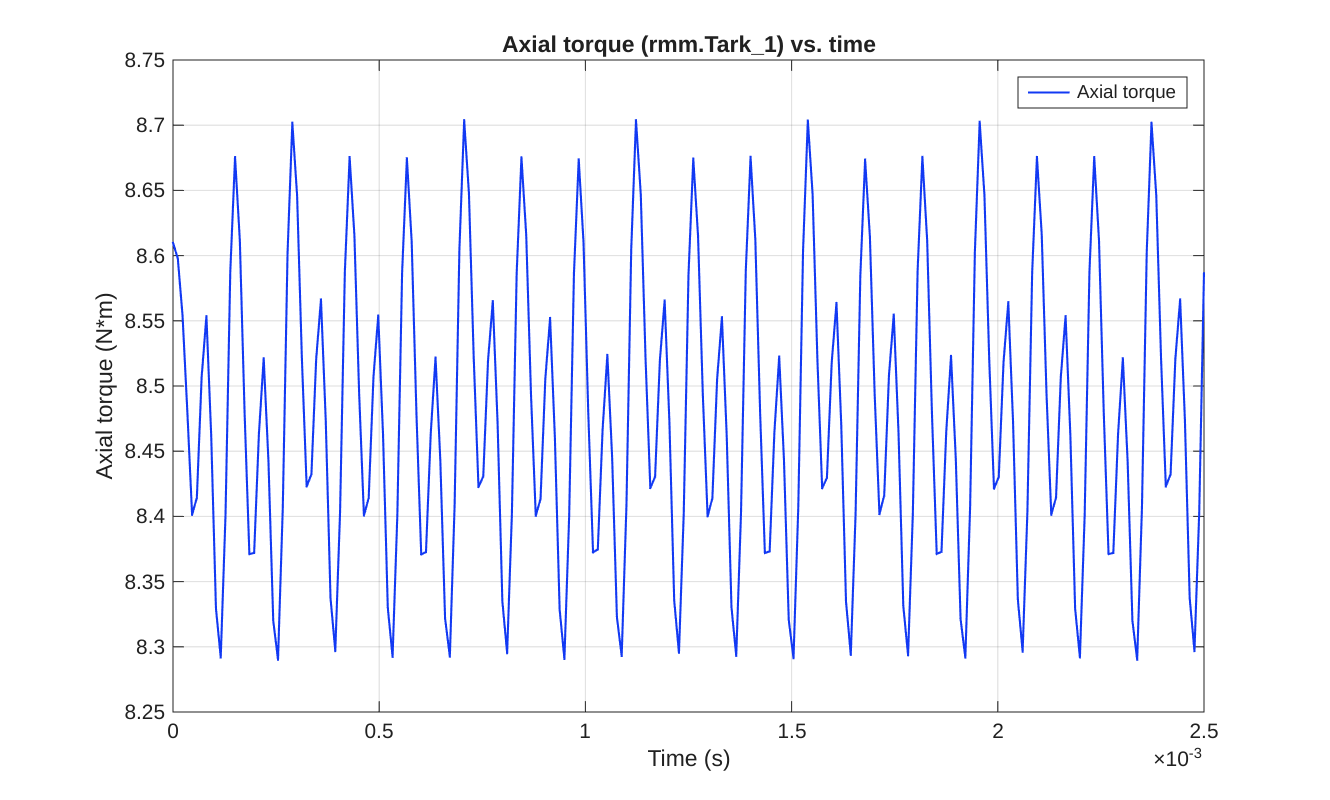
\includegraphics[width=\columnwidth]{figures/torque.png}
\caption{Axial torque (\texttt{rmm.Tark\_1}) over the time-dependent sweep.}
\label{fig:fem_torque}
\end{figure}

\begin{figure}[!htbp]
\centering
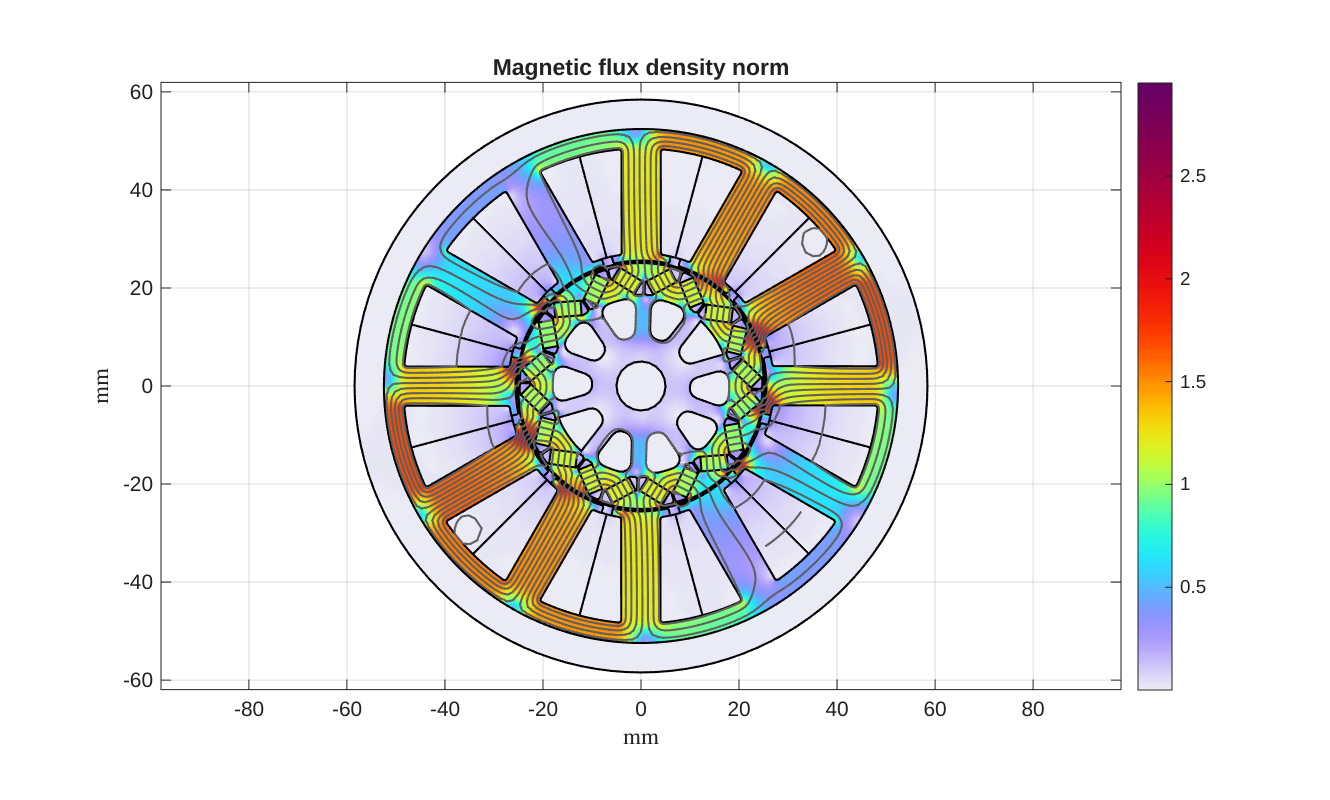
\includegraphics[width=\columnwidth]{figures/flux_density.png}
\caption{Magnetic flux density norm with field lines, at the swept operating point.}
\label{fig:fem_flux}
\end{figure}

\begin{figure}[!htbp]
\centering
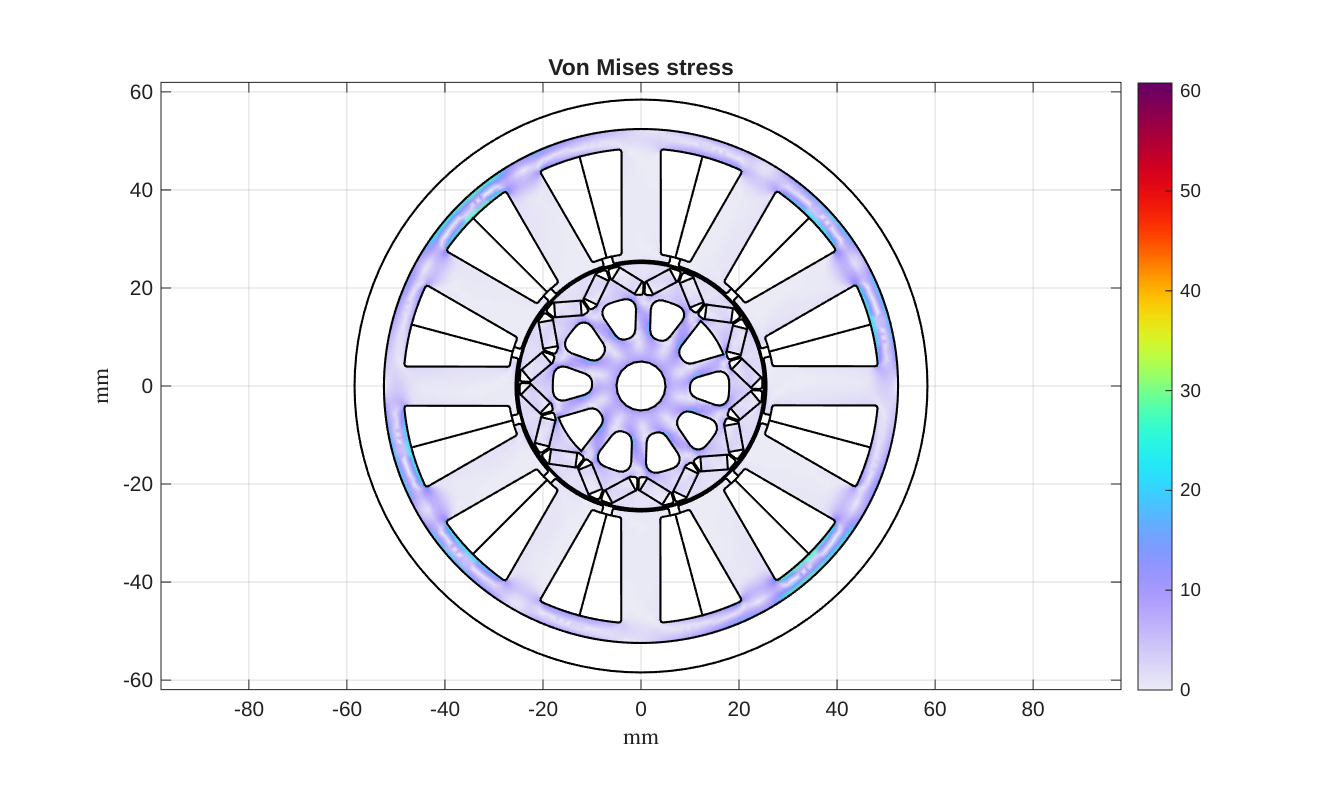
\includegraphics[width=\columnwidth]{figures/von_mises_stress.png}
\caption{Von Mises stress distribution from the coupled structural solve.}
\label{fig:fem_stress}
\end{figure}

\begin{figure}[!htbp]
\centering
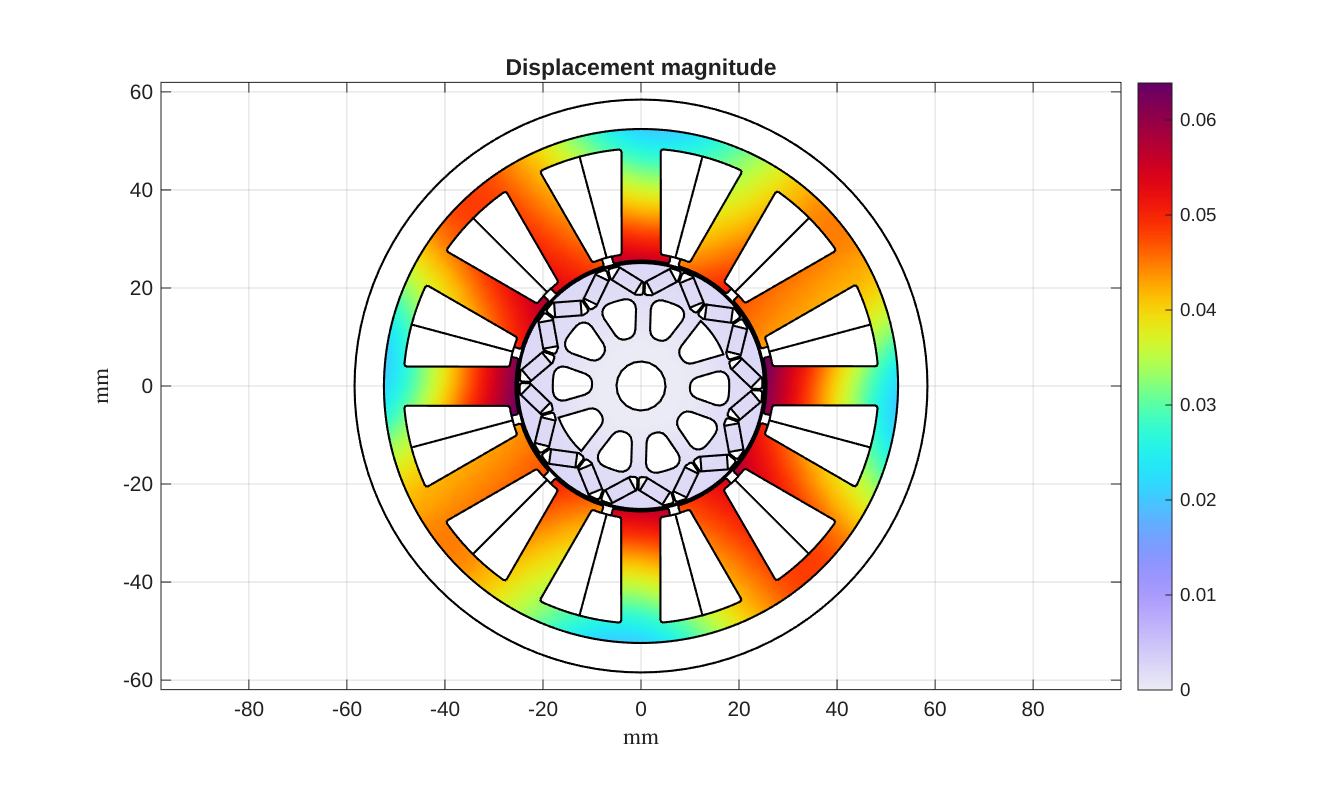
\includegraphics[width=\columnwidth]{figures/displacement.png}
\caption{Displacement magnitude from the coupled structural solve.}
\label{fig:fem_displacement}
\end{figure}

\subsection{Energy Efficiency Map}
\label{sec:efficiency_map}
\texttt{EfficiencyMapSizer.m} builds a rough analytical loss model directly from the converged \texttt{IPMRotorSizer} geometry and winding data, and sweeps it over the achievable torque-speed envelope. At the rated point it draws the same current pushed into the FEM above ($I_{pk}=74.2\,\text{A}$) from the identical $I_q=T/(1.5\cdot(P/2)\cdot\Psi_{PM1})$ formula (eq.~\ref{eq:iq_current}); this is a from-construction match, not an independent FEM cross-check (no FEM-derived efficiency or loss figure exists to compare against yet):
\begin{itemize}
    \item \textbf{Copper loss:} phase resistance from a geometric mean-turn-length estimate (twice the stack length plus a semicircular end-turn bridging one slot pitch on each end, appropriate for this design's non-overlapping, single-tooth-wound coils, \sectionname~\ref{sec:pole_slot_number}), evaluated at an assumed $100\,\text{\textdegree{}C}$ hot winding temperature. This gives $R_s\approx604\,\text{m}\Omega$/phase over a $1.22\,\text{kg}$ stator core (teeth+yoke).
    \item \textbf{Core loss:} a two-term (hysteresis+eddy) Steinmetz fit calibrated to the M235-35A lamination's single datasheet point ($P_{1.5/50}=2.35\,\text{W/kg}$, literally what ``235'' means in the EN\,10106 grade name), extrapolated up to this design's much higher electrical frequency ($f_c=1020\,\text{Hz}$, a $20\times$ extrapolation past the 50\,Hz reference point). This extrapolation is flagged as the map's single biggest source of uncertainty; treat core-loss numbers as order-of-magnitude, not precise.
    \item \textbf{Excluded:} mechanical (windage/bearing) losses; no validated model at this design stage.
\end{itemize}
At the rated point (9.8\,Nm, $n_{base}=12{,}240$\,rpm, $I_{pk}=74.2$\,A, the same current validated by FEM above), this gives $P_{cu}\approx4.99\,\text{kW}$, $P_{fe}\approx0.33\,\text{kW}$, and an efficiency of $\approx70\%$. This is markedly lower than the $\eta=0.92$ assumed in \sectionname~\ref{sec:part_b_fea}'s electromechanical power modeling, and traces directly to the same flux-linkage shortfall discussed throughout Part A and \sectionname~\ref{sec:sim_framework}: with $\Psi_{PM1}$ under target, more current ($I_{pk}=74.2\,\text{A}$, eq.~\ref{eq:iq_current}) is needed to produce the same torque than a fully-fluxed design would need, which raises $I^2R$ loss directly. Closing the leakage-model gap (README.md's ``Known issues'' section) is therefore not just a torque/flux-linkage fix; it is the single highest-leverage change for this design's actual efficiency.

\figurename~\ref{fig:efficiency_map} sweeps this loss model over the full torque-speed grid ($T\in[0,9.8]\,\text{Nm}$, $n\in[0,14{,}400]\,\text{rpm}$, the design's own continuous rating and inverter-limited speed cap), with $I_d=0$ below corner speed (matching \sectionname~\ref{sec:ricca_methodology}'s own corner-point assumption) and a simplified voltage-limited flux-weakening solve above it. The narrow infeasible band immediately above corner speed is a direct, honest consequence of the same flux-linkage shortfall: at this design's actual (low) $\Psi_{PM1}$, sustaining full torque needs more current than the voltage budget allows once speed rises even slightly, so this map's flux-weakening range is narrower than the $1.18\times$ ratio \sectionname~\ref{sec:corner_speed} targets. The assignment's peak-torque (5\,s, $21.5$\,Nm) and spec max-speed ($20{,}000$\,rpm) targets are marked for context only; neither is evaluated by this continuous-duty loss model.

\begin{figure*}[!t]
\centering
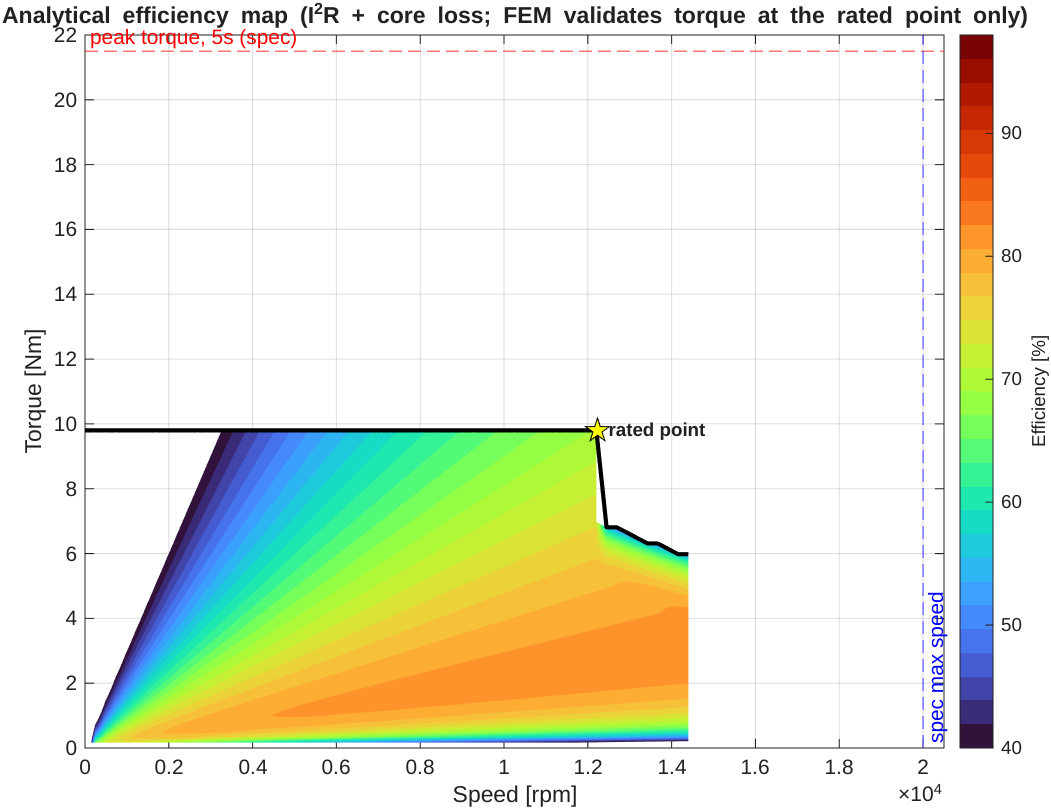
\includegraphics[width=0.75\textwidth]{figures/efficiency_map.png}
\caption{Analytical efficiency map over the torque-speed envelope (\texttt{EfficiencyMapSizer.plotMap}). Black line: achievable envelope. Star: rated design point.}
\label{fig:efficiency_map}
\end{figure*}

\section{Thermal and Mechanical Analysis}
\label{SEC:Thermal}
A critical design constraint is the existing \textbf{4\,l/min liquid cooling loop}, originally sized for the current motor's 12.4\,kW rating. The mechanical side of this section is already covered by full FEM in \sectionname~\ref{sec:sim_framework} (peak von Mises stress and displacement, \tablename~\ref{tab:fem_results}); this section covers the thermal side, which stops short of a full thermal FEM or lumped-parameter model in this design iteration, not for lack of a COMSOL path (the same coupled-study template already used for the structural side supports a thermal physics interface), but because closing the leakage-model gap (\sectionname~\ref{sec:sim_framework}) comes first: the loss figures below are downstream of $I_{pk}$, which is itself inflated by the same flux-linkage shortfall, so a thermal model built now would need re-solving once that's fixed.

The analytical loss model from \sectionname~\ref{sec:efficiency_map} puts total loss at the rated point at $P_{cu}+P_{fe}\approx5.32\,\text{kW}$ ($4.99$\,kW copper, $0.33$\,kW core) against an $\approx$12.6\,kW mechanical output (\tablename~\ref{tab:motor_design_data}) ; a substantial heat load, dominated by copper loss, and itself inflated by the same flux-linkage shortfall discussed throughout this report (\sectionname~\ref{sec:corner_speed}, \sectionname~\ref{sec:efficiency_map}). Whether the existing 4\,l/min loop can hold this load within the magnets' demagnetization limit and the winding insulation's temperature class depends on convective/conductive thermal resistances not modeled here; sizing a lumped-parameter or thermal-FEM model against this loss figure is the natural next step before the design can be considered thermally validated. The $140\,\text{\textdegree{}C}$ PM operating temperature already assumed in \sectionname~\ref{sec:magnet_material} (and the resulting need for a high-temperature-stable magnet variant) reflects an expectation that this loss level runs hot, not a validated steady-state result.

\section{Conclusion}
\label{SEC:Conclusion}
Starting from the current 10-pole/12-slot DD5-14-10-POW motor and its inverter-limited 1.1 flux-weakening ratio (\sectionname~\ref{sec:Inverter}), Part A defined boundary requirements (\tablename~\ref{tab:propulsion_motor_requirements}) and, keeping the pole/slot count for its proven cogging-torque and winding benefits (\sectionname~\ref{sec:pole_slot_number}), sized a V-shape IPM rotor targeting $L_q>L_d$ for added reluctance torque. Two independent Esson's-rule estimates (\sectionname~\ref{sec:ricca_methodology}) bracket a feasible bore/stack-length envelope inside the 120\,mm/110\,mm boundary, and the full Di Gerlando \& Ricca sizing procedure (\texttt{IPMRotorSizer}) converges end-to-end for this design point, giving a complete geometry, winding, and rated operating point (\tablename~\ref{tab:motor_design_data}) together with a rotor-bridge stress check that is comfortably safe at the 14,400\,rpm operating cap (\sectionname~\ref{sec:bridge_sizing}).

Part B (\sectionname~\ref{sec:part_b_fea}) exercised this pipeline end-to-end: \texttt{ComsolPrebuiltInterface} pushed the converged design into the prebuilt COMSOL model and ran the coupled EM/structural transient study, giving $8.48\,\text{Nm}$ average torque ($4.9\%$ ripple), $63.0\,\text{MPa}$ peak von Mises stress, and $0.069\,\text{mm}$ peak displacement (\sectionname~\ref{sec:sim_framework}, \tablename~\ref{tab:fem_results}) ; structurally safe with margin, though the torque undershoots the $9.8\,\text{Nm}$ analytical target for the reason discussed below. An analytical loss model (\sectionname~\ref{sec:efficiency_map}) additionally swept the full torque-speed envelope, giving the energy efficiency map and a quantified rated-point efficiency of $\approx70\%$.

Two related open items should be resolved before the design is considered converged: (1) the no-load leakage constant inside \texttt{IPMRotorSizer} is calibrated to the reference paper's larger pole pitch and underestimates leakage by roughly 4--6$\times$ at this project's tighter 10-pole/12-slot geometry (README.md's ``Known issues'' section), which is the most likely cause of the required flux linkage $\Psi_m\approx0.0426$\,Wb (\sectionname~\ref{sec:corner_speed}) not yet being met by the converged $\Psi_{PM1}=0.0176$\,Wb ; and, now quantified, the direct cause of the FEM torque shortfall (\sectionname~\ref{sec:sim_framework}) and the $\approx70\%$ rated-point efficiency (\sectionname~\ref{sec:efficiency_map}), since hitting the intended torque with too little flux means drawing more current than planned, at a direct $I^2R$ cost; and (2) the resulting stator outer diameter ($D_{es}=108.8\,\text{mm}$) still exceeds the old motor's own 89.9\,mm stator-core OD (\sectionname~\ref{sec:current_motor_background}) by about 19\,mm, though it remains within the 120\,mm boundary requirement including cooling. Closing the leakage-model gap first is the natural next step, since it directly affects all three figures.

Beyond these two physics-model gaps, several items from the assignment brief and \tablename~\ref{tab:propulsion_motor_requirements} were carried into this report's boundary-requirements table but never closed by a later design or verification step in this iteration, and are flagged here rather than left silently unaddressed: total motor weight and the resulting power density (only a partial 1.22\,kg stator-core mass is ever computed, \sectionname~\ref{sec:efficiency_map}; rotor core, magnets, windings, shaft, and housing are not summed, so compliance with the $\leq$2800\,g / $\geq$10\,kW/kg targets is currently unknown), IP65 sealing, hub compatibility, the three-phase cable diameter, all three sensor requirements (rotor position, stator temperature, rotor temperature), the cooling-circuit routing (beyond inheriting the existing liquid loop), and the rotary-encoder/output-spline shaft-interface compatibility. Assignment A's own task to evaluate reducing or adding gearbox stages is likewise not carried out: the existing 14:1 ratio is kept as a given (\sectionname~\ref{sec:current_motor_background}) rather than examined as a mass/volume trade-off against the motor. None of these affects the electromagnetic/structural results already validated above, but they remain open scope for a future iteration.

\bibliographystyle{IEEEtran}
\bibliography{IEEEabrv,references}

\end{document}
